\cotefile{109}
\scanpage{9}
\hfill\uline{Terminology}

\diagram{\small\begin{tabular}{@{}p{.72\linewidth}@{\quad}l@{}}
\inserted{primitive,} primary, secondary, ternary\ldots\ structure & 4.\\
standard type (iterated fibre products of) & 5.\\
$n$-stacks, $\infty$-stacks, \deleted{\unsure{an|en|n}} $n$-$\underline{C}$-stacks & 13.\\
Coherator & 13\\
Hot-equivalence of site structure & 25\\
\hspace{1.5em}test category(!)\ \hrulefill & 26, \uline{39}\\
test-topology & 27\\
$\left.\begin{array}{@{}l@{}}
\text{modelizer !/ model-preserving}\quad\deleted{\underline{41}}\\
\hfill\text{(or modelizing) functor !}
\end{array}\right\}$ &
\begin{minipage}{.22\linewidth}
\diagram{\begin{tikzcd}[ampersand replacement=\&,row sep=.1em,column sep=.55em]
{} \& \underline{41}\\
28 \arrow[ur] \arrow[dr] \& {}\\
{} \& \underline{42}
\end{tikzcd}}
\end{minipage}\\
$\left.\begin{array}{@{}l@{}}
\text{'basic modelizer (Cat)}\\
\text{elementary modelizer(\unsure{!,|!})}
\end{array}\right)$ & $29^7$\\
\uline{Strict} test. category \deleted{\unsure{(!)|!|4.}} & 33, 39\\
standard simplices\quad\textemdash\ \textemdash\ \hrulefill & \\
\hspace{4em}cubes & 34\\
% Both drawings are canceled; their actual cancellation strokes are reproduced in TikZ below.
\begin{minipage}{.4\linewidth}
\figure{
\begin{tikzpicture}[x=.26cm,y=.26cm,line cap=round,line join=round]
\draw[line width=.7pt] (0,0) -- (-.06,1.22) -- (1.13,1.26) -- (1.19,.12);
\draw[line width=1pt] (.06,.1) -- (.2,-.02) -- (.9,.03);
\draw[line width=.7pt] (.25,1.09) -- (.27,.04) .. controls (.19,-.12) and (-.02,-.08) .. (.07,.04);
\draw[line width=.7pt] (.25,.4) -- (1.19,1.6) (.25,.43) -- (.93,1);
\node at (1.58,-.01) {,};
\draw[line width=.7pt] (2.04,.05) -- (2.01,1.4) -- (3.54,1.46) -- (3.59,.05) -- cycle;
\draw[line width=.7pt] (2.18,1.32) -- (2.2,-.02) (2.04,.4) -- (3.09,.89);
\draw[line width=.8pt] (1.35,.74) .. controls (1.86,1.25) and (2.51,2.16) .. (2.72,2.19) .. controls (2.9,2.25) and (3.03,1.84) .. (3.5,2.1) -- (3.12,1.98) -- (2.05,.46);
\draw[line width=.75pt] (3.66,1.16) -- (3.02,.13) .. controls (2.77,-.37) and (3.22,-.15) .. (3.96,.41);
\end{tikzpicture}}
\end{minipage} & \deleted{34}\\
$\left.\begin{array}{@{}l@{}}
\text{aspheric (topos, object of topos, \inserted{map of objects})}\\
\text{locally \uline{aspheric topos, tot.\ asph.\ topos}}
\end{array}\right)$ & 35\\
% The visible opening parenthesis has no matching closing parenthesis.
\uline{Weak equivalence} ($f:X\mathrel{\unsure{-|\to}}Y$ m; of topos & ?\\
homotopy interval & 37\\
{}[strict] elementary modelizer & 39.\\
$\left.\begin{array}{@{}l@{}}
\text{local test catégory}\\
\text{local el.\ modelizer}
\end{array}\right)$ & 39\\
{}[locally] modelizing topos & 39
\end{tabular}}
% archive sheet number: 8

\scanpage{10}
\begin{center}Reflexions Mathématique\end{center}

(The simplest thing \inserted{for me} is to write out a\deleted{\unsure{n}} \inserted{possible} alternative version as our photocopy of the original is not that clear now. I'll underline in red places where the words are changed from your original whether by Breen or by us.)

After a twelve years' silence, the time has come for the author's works of maturity, with his vision and style renewed. Here is \uline{a} day-by-day account of an explorer's \deleted{travel} \inserted{\uline{journey}} with occasional reflections on the travel \uline{itself} \unsure{((|(}as well as on the traveler and the \uline{manifold} world around \uline{him},) \inserted{thus} recapturing its genuine nature: \uline{that} of an impassioned adventure, rooted in life

In the two forthcoming volumes, under the common title ``Pursuing Stacks'' (the first volume of which is subtitled ``The Modelizing Story,''), the author sketches some themes of a vast sythesis of homotopical algebra, (co)homological algebra and topos theory -- ripe now for more than fifteen years \uline{but} never yet begun. The leading thread, tenacious and omnipresent (while often remaining implicit) comes from algebraic geometry, and from the intuitions (rich precise and provocat\uline{ive}ly fragmentary) \uline{surrounding} the notions of sheaves, stacks, $2$-stacks ``etc.'' on a topos.

Thes two volumes are the first in a planned, considerably wider series of ``Réflexions Mathématiques'' \uline{in which} the author intends to \uline{present}, among other things, some ``naive ideas'' about two ``new continents'', eager to be discovered and explored. One \uline{stems from}
% archive sheet number: 9

\scanpage{11}
a suitable notion of a ``tame'' topological space, viewed as the natural set-up for expressing and stimulating the topological intuition of shape and form, which for so long has been squeezed \uline{into} the straitjacket of a ``General Topology'' tailored for the use of the analyst, not for geometry. This is inapt notably (because of pervasive ``wildness'' phenomena) for \uline{\inserted{the} study\deleted{ing} \inserted{of}} homotopy types of spaces of homeomorphisms, imbeddings \& the like, or for developing a comprehensive ``dévissage'' theory of stratified structures (whereas such structures \deleted{abound} \uline{crop up everywhere} notably in any question of ``moduli'' \deleted{\unsure{of}}for geometrical configurations capable of continuous variation and giving rise to degeneracy phenomena). The other continent appears \uline{at} the confluence of a multitude of streams of thought and insights, coming from topology, conformal geometry, algebraic geometry, discrete and profinite groups, algebraic groups over number fields, regular polyhedra, arithmetics, ``motives''\ldots, \uline{called together for} the exploration of the action of profinite ``absolute'' Galois groups (such as $\operatorname{Gal}_{\overline{\mathbb{Q}}/\mathbb{Q}}$) on certain (so called ``anabelian'') profinite geometrical fundamental groups (such as $\pi_{1}(P_{\overline{\mathbb{Q}}}-\{0,1,\infty\})$,

One of the leading threads comes from the combinatorial topology

(Continues without change until last paragraph)

The \inserted{two} first \deleted{\unsure{two}} volumes ``Pursuing Stacks'', started\textendash{} through the impetus of a correspondence in English are written in that language. They begin with a substantial common introduction \uline{of which a first part}, of personal rather than technical character, is written in French (the author's adopted language.).
% archive sheet number: 10

\scanpage{13}
\begin{center}\uline{COMMENTS ON ``PURSUING STACKS''}\end{center}

\diagram{\begin{tabular}{@{}l@{\quad}l@{}}
p2 $\ell$8 & inadequate\\
p2-$\ell$-15 & incomplete\\
p3 $\ell$-8 & pertinent\\
p4 $\ell$6 & indiscriminate\\
\hspace*{1.45em}$\ell$-1 & misled\\
p4-$\ell$-16 & arbitrary\\
\hspace*{1.45em}$\ell$-8 & the same\\
\multicolumn{2}{@{}l@{}}{Section 14 etc}\\
p2 $\ell$18 & impediment\\
p3 $\ell$4 & CW-spaces\\
\hspace*{1.45em}$\ell$12 & have\\
\hspace*{1.45em}$\ell$15 & adequate
\end{tabular}}

p3\qquad The question of cubical versus simplicial sets is an interesting one. The category of simplicial sets has a number of good properties, which have made it very popular.

1.\quad It is cartesian closed.

2.\quad The realisation functor gives an equivalence between the homotopy category of Kan simplicial sets and the homotopy category of CW-spaces and the proof of this has been published.

3.\quad The realisation functor satisfies $\lvert X\times Y\rvert$ is homeomorphic to $\lvert X\rvert\times\lvert Y\rvert$ (at least if one takes the fine topology with respect to compact subsets on the latter product, as is the correct thing to do for other purposes, such as obtaining the right cartesian closed category for topological spaces). Also simplicial sets are firmly embedded in the literature. Again, there is a Dold-Kan theorem, giving an equivalence between chain complexes and simplicial abelian groups. A neat proof of the Serre spectral sequence using simplicial methods has been published by A. Dress (see the reference in my paper with Heath ``Cogluing homotopy equivalences'').

By contrast, cubical sets are not greatly used in the literature, although a number of writers have found them convenient. A recent exposition by Massey of singular homology theory uses the cubical method throughout, and finds them very convenient. Again, Brown-Higgins have found them essential for their methods. The difficulties about using them are that they are not firmly embedded in the
% archive sheet number: 12

\scanpage{14}
\mspage{2}% typed -2-
literature. The proof of the equivalence of homotopy categories is not in the literature, indeed there is just this M.Phil. thesis of F. Hintze at Warwick which gives full details. (Part of the proof is also given by Federer in notes on algebraic topology from Brown University, 1962.) Cubical sets have a cartesian product, which does not have the correct realisation. This causes all sorts of difficulties. There is a tensor product which has the correct realisation, but having two products certainly complicates the issues. To obtain a Dold-Kan theorem, one has to introduce extra structure on cubical sets, namely the connections considered by Brown-Higgins. Realisations when you have this extra structure have not yet been worked out. More general notions of cubical groups, and related constructions, which have been well worked over by Kan and others in the simplicial case, have not yet been worked out for cubical groups.

$\ell$-3\qquad and \uline{a} corresponding.

p4 $\ell$8\qquad I would prefer here to talk about the Dold-Kan theorem, since Puppe only came in at a later stage, after the theorem had been proved independently by Dold and Kan. In fact Dold's original version was rather computational, and it was Kan who pointed out that the functor from chain complexes to simplicial abelian groups is given in a dimension $n$ by $\operatorname{Hom}(C_{N}\Delta^{n},C)$ for a chain complex $C$ . Also, a description of the theorem for a general additive category was done by Epstein.

It is curious that the way the Loday approach to homotopy type has gone is via $n$-simplicial sets although the proof of the modelling of all homotopy types is as yet incomplete. Similarly, the general van Kampen theory of Brown-Loday uses $n$-fold groupoids, more particularly $\mathrm{Cat}^{n}$-groups . I wonder whether the main problem is that to define gadgets like these for other situations, such as topoi, it may be necessary to have unit interval constructions, and this is where the various stack structures intervene, before obtaining the $\mathrm{Cat}^{n}$-groups.

$\ell$-7\qquad Replace eluding by evading.

$\ell$-2\qquad developed

p5 $\ell$8,9\quad Maybe it would be better as ``whereas it seems to me we have now come to a definite starting point''.

$\ell$11\qquad manifold

p7\qquad This construction of the nerve and its relation to homotopy types has been studied in detail by Fritsch and Latch.

p8\qquad The middle paragraph of this page is interesting. Certainly finding categories which model geometric situations, and then by the nerve obtaining a topological
% archive sheet number: 13

\scanpage{15}
\mspage{3}% typed -3-
space, has been found a very useful tool in geometric topology, particularly in recent work on the algebraic $K$-theory of topological spaces, by Waldhausen, and others. But it is fair to say that at this time it has not proved a \textit{basic} tool, and has not led itself to computation. An interesting test case is to try and determine $\pi_{3}(S^{2})$ without knowing about the Hopf fibration $S^{1}\to S^{3}\to S^{2}$ .

p9 $\ell$-5\qquad developing

p10 $\ell$6\qquad misled

$\ell$-15\quad standard. In many places, standart is used instead of standard.

p11 $\ell$10\quad the formal analogy

$\ell$12\qquad developing

$\ell$13\qquad standard

p12 $\ell$19\quad standard. Similarly lower down the page.

p13\qquad Isn't the reason that the category of all groupoids is not a topos is that it does not have a sub-object classifier?

p15 $\ell$18\quad Maybe omit ``still about''

p16 $\ell$11\quad ``This recalls to mind of course Quillen's''

$\ell$-5\qquad such a category

p17 $\ell$-2\quad commute with formation

\handwritten{so far, so good!}
% archive sheet number: 14

\scanpage{17}
\begin{center}Errors in 1\textsuperscript{st} 100 pages of notes + letter to Quillen.\end{center}

\uline{Quillen letter:}

``Commute with'' not ``commute to'' e.g p.5 line 14 - repeated.

Page 5 line 15 - ``including the structure of categories, groupoids\ldots.'' would be more normal.

Page $5'$, line 11, - ``standard'' not ``standar\deleted{d}t'' - repeated.

line -16, ``having \uline{the} same objects'' - article is missing

Page $6'$, line -13, ``each of the categor\uline{ies}''

\uline{Re}fle\uline{ctions}

Page 1, line -13\quad ``indispensable''

2 line 18\quad ``impediments''

5 line 11\quad ``manifold'' - would be more usual

8 line - 8\quad ``adequate''

9 line 11\quad ``indispensable''

16 line 11\quad ``reminds'' needs an object eg. ``me'' or ``one''

21 line 12\quad ``$n$-tuples'' is I believe correct.

27 line -14\quad ``how can one define''

32 line 17 (middle of page) probably `modelizer''

34 line 6\quad ``which allow\ldots'' this phrase is not clear in sense.

``Allow'' with ``to'' usually takes an object i.e ``which allow one to\ldots'' but this doesn't seem to be right here

``Allow for'' is different.

39 line 18-``is'' not ``be''

41 line -6\quad ``we have'' is more correct than ``we got'' - which is American - $\therefore$ more like 16\textsuperscript{th} \unsure{or|\&} 17\textsuperscript{th} century English!
% archive sheet number: 16

\scanpage{18}
Page \deleted{\unsure{3|2}}41 \unsure{-}line -4\quad ``aspheric'' not ``asperic'' (avec\unsure{,|-} les asperges !\unsure{..|''})\unsure{..|.}

42, line -3, ``analogues'' would be more usual.

55 line 12, ``rather than just \uline{to} take $B$ and \uline{to} keep\ldots''

59 line -12, ``denote'' not ``debote''

60 line -11, ``of'' not ``ob''

61 line -20, ``Assume'' not ``Asumme''

63 line 16\quad ``make sense'' or ``have a sense''

66 line 13\quad I'm no \unsure{Latin|latin} expert but isn't it rather \unsure{Compositum|compositum} (singular) composita (plural) than composita, compositae ? My \unsure{Latin|latin} dictionary isn't \unsure{goodenough|good enough} to be sure !

p.77 line 12\quad ``isn't'' not ``is'nt'' this is repeated several times in different forms e.g ``does'nt'' for ``doesn't''

p.87 line 8\quad ``we \uline{have} only got to\ldots'' or ``we have only to\ldots''

p88 line 2\quad ``does'nt'' should be ``doesn't''; there is also an is'nt lurking \unsure{aroundhere|around here}.

p.89 line 3\quad ``to have got me'' or alternatively \unsure{‘|``}to have made me''

line 8\quad is ``very'' necessary?

line -15\quad \unsure{‘|``}last not least’ is more usually \unsure{‘|``}last but not least''; an alternative would be ``last, not least,''.

P.90 line -15\quad ``compare'' takes ``with'' as does commute (4 occurences on this page)

line -9\quad some more ``is'nt''s .

line -8, replace ``,'' by ``that'' - this would give a better flow of words.
% archive sheet number: 17

\scanpage{19}
\mspage{2}% handwritten -2-

p.91 line 1. ``in view of\unsure{''|'} indicates a result of previous happenings

``with a view to'' indicates future hopes \& expectations

lines 15 \& 16 ``we've got'' or ``we have got'' is better.

line -16. ``avatars'' not ``avators''

p.92 line -16 probably ``informal'' is what you want (repeated in line -3)

p-99. $X$ and $Y$ have changed to $F$ \& $G$ it seems

p.100 line -16, ``having \uline{the} same objects''

% archive sheet number: 18

\scanpage{21}

\tikz[remember picture,overlay]\coordinate (scxxitop);\unsure{p.} \unsure{77|11} line 12 \unsure{isn't|is'nt} \unsure{not} \unsure{is'nt|isn't} \unsure{--} \illegible{3} \unsure{er} form later (i.e ``does'nt'' is used for ``doesn't'')

\tikz[remember picture,overlay]\coordinate (scxxifainttop);p.87 line 8 ``we \uline{have} only got to'' or ``we have only to\unsure{..-|...|..}''

p.88 line 2 ``does'nt'' should be ``doesn't'' (``is'\tikz[remember picture,overlay]\coordinate (scxxia);nt'' occurs \deleted{\unsure{a|a l}}a bit further down

p.89. line 3 ``to have got me'' or alternatively ``to have made me''

line 8 ``is ``very'' necessary?

\deleted{p.} line -15 ``last not least'' is more usually ``last but not least'' an alternative would be ``last, not least,''

p.90 line -15 ``compare'' takes ``with'' as does ``commute\tikz[remember picture,overlay]\coordinate (scxxib);'' \margin{\tikz[baseline=(m.base)]{\node[inner sep=1pt,text width=2cm,align=left](m){(4 occurences on this page)}; \draw (m.west) to[bend right=10] (m.south west) -- (m.south east);}}

\deleted{also this line -15 has a double negative}

\deleted{not -- neither} ``isn't line -\deleted{\unsure{4|14}}9 (twice)

line -8 replace ``,'' by ``that'' - would give better flow of words

p.91 line 1 ``in view of'' indicates a result of previous happenings

``with the view to'' indicates future hopes \& expectations.

line ``we've got'' or ``we have got'' (``We got'' is used in standardish English. \deleted{only} in phrases like \deleted{``we got into the car'' \unsure{or}} ``We got a loaf of bread and then ate it'', the conditional ``if we ...'' always takes ``have'')

\tikz[remember picture,overlay]\coordinate (scxxifaintbottom);\deleted{p} line -16 ``avatars'' not ``avators''

p.92 line ``-16'' probably ``informal'' (repeated line -3)

p.99. \tikz[remember picture,overlay]\coordinate (scxxic);$X$ \deleted{ha} $Y$ have got changed to $F, G$ it seems.

p.100 line -16 ``\tikz[remember picture,overlay]\coordinate (scxxid);having \uline{the} same objects''

\margin{Sent 19/12/83}

\figure{\begin{tikzpicture}[remember picture,x=.92\linewidth,y=1ex]
\draw[overlay,gray,thin] (scxxia) -- (scxxic);
\draw[overlay,gray,thin] (scxxib) to[bend left=2] (scxxid);
\draw (0.625,2.2) .. controls (.633,2.65) and (.638,2.45) .. (.643,2.42) .. controls (.649,2.32) and (.653,2.65) .. (.658,2.55);
\draw (.644,2.45) -- (.645,2.95);
\draw (0,.4) .. controls (.10,.9) and (.17,-.4) .. (.32,0) .. controls (.57,.9) and (.72,-.3) .. (.89,.75) .. controls (.94,.9) and (.98,.65) .. (1,.4);
\end{tikzpicture}}

p.102 line -1, \unsure{`|``}commute \uline{with}'' again

p.105 line 7 ``developing'' (single p.)

p.107 line 5 ``is'nt'' again replace by ``isn't'' also \inserted{in} line -5.

line 14 ``saturation'' \deleted{\unsure{t}}-

line -3 ``K\raisebox{1.1ex}[0pt][0pt]{\makebox[0pt][l]{\deleted{\unsure{h}}}}an'' not ``\unsure{Khan|Khân}''

p109 line -9 ``isn't''

p.111 line 19 ``relation\uuline{s}hips''.

p.112 line 14, ``we'll say we've got''

p.113 line 15 ``commute with'' repeat line -15

line -14 ``we've got'' or simply ``we have''

\tikz[remember picture,overlay]\coordinate (scxxibottom);p.115\unsure{:} line -5 \& 6, ``commute with''

\figure{\begin{tikzpicture}[remember picture,overlay]
% Visible side rules and the fainter partial rule at far left.
\coordinate (scxxileftedge) at ([xshift=-.5em]scxxitop);
\coordinate (scxxirightedge) at ([xshift=.92\linewidth]scxxitop);
\coordinate (scxxifaredge) at ([xshift=-5em]scxxitop);
\draw[overlay,thin] ([yshift=1ex]scxxileftedge) -- ([yshift=-2ex]scxxileftedge |- scxxibottom);
\draw[overlay,thin] ([yshift=1ex]scxxirightedge) -- ([yshift=-3ex]scxxirightedge |- scxxibottom);
\draw[overlay,gray,very thin] (scxxifaredge |- scxxifainttop) -- ([yshift=3ex]scxxifaredge |- scxxifaintbottom);
\end{tikzpicture}}

% archive sheet number: 20

\scanpage{22}
\tikz[remember picture,overlay]\coordinate (scxxiitop);

p.116 line -6, $\unsure{R|K}_h\subset\unsure{R|K}_n$\raisebox{-1.1ex}{\unsure{''}} should be $R_h\subset\Sigma_h$.

p117 line 11 \& 12, commutation .... with.''

line -17 ``I'd better assume ...''

p.119 line 5, \tikz[baseline=(word.base)]{
\node[inner sep=0pt,anchor=west](word) at (3.25,0){``onto''};
\node[draw,rounded corners=5pt,inner sep=2pt](add) at (1.45,0){\inserted{\unsure{``}not ``unto''}};
\coordinate (tip) at ([xshift=1.3em]word.east);
\draw[->] (add.south east) .. controls +(0.45,-.42) and +(.17,-.65) .. (tip);
\draw ([xshift=-.6ex,yshift=-.2ex]tip) -- ([xshift=.4ex,yshift=.6ex]tip) -- ([xshift=.8ex,yshift=-.5ex]tip);
}

line 14 ``allows \uuline{one} to''

p114 \& 115 handwritten comment: is \S52 intended rather than \S51.

\tikz[remember picture,overlay]\coordinate (scxxiiendows);p.121 line -17 ``endows''

\reversemarginpar
\margin{\tikz[baseline=(cancelref.base)]{
\node[inner sep=0pt](cancelref){\deleted{\unsure{?} \unsure{*} p122 \unsure{?}}};
\draw[line width=.45pt] ([xshift=-.25em,yshift=-.35ex]cancelref.west) -- ([xshift=.25em,yshift=.15ex]cancelref.east);
\draw[line width=.45pt] ([xshift=-.35em,yshift=-.6ex]cancelref.west) -- ([xshift=.05em,yshift=.45ex]cancelref.east);
\draw[line width=.35pt] ([xshift=.65em,yshift=-.75ex]cancelref.west) -- ([xshift=-.1em,yshift=-.15ex]cancelref.east);
}}
\normalmarginpar

p.123 \deleted{\unsure{l}}line 9 ``standard''

line 13 ``with direct sums'' line -1 ``commutes with''

p.124 line 17 ``a long time ago''

p128 line \deleted{\unsure{16}}-12 ``standard''

p131 line 16 ``commutes with'', line 18 ``it is''

p132 line -14 `wasn't''

133 line 13 (handwritten \unsure{?}) ``commutes with'

p.135 line 4, commas needed around ``,of course,''

137 line -13, ``wasn't''

138 line -15 ``through'' line -5 ``standard''

p140 line \deleted{\unsure{3}}4 ``commutes with'',

141 line -1 ``standard''

142 line 15 $s_1=\delta_0$. line -15, ``allow one to''

p.146 line -3, ``usual'' \deleted{does} line -1 ``doesn't or shouldn't''

147 \deleted{st} line 2 \unsure{``|`}standard' line 10 ``commutes with'', line 18 ``doesn't''

line 20\unsure{.|,} \unsure{``|`}with' not to''

148 line 21 ``developed'' line -1. ``standard.''

149. ``line 7 ``standard'' line 12 ``isn't''

\tikz[remember picture,overlay]\coordinate (scxxiip);p.151 line 8 ``isn't'', line 17 ``a long time ago'' line 18 ``putting off'' would be more usual.

p.152 line 17 ``developed''.; line -10. ``lead to develop''; line -9 ``\deleted{\unsure{allow}} ``which will allow us to define''

\tikz[remember picture,baseline=(n.base)]{\node[inner sep=1pt](n){151}; \draw[rotate around={32:(n.center)}] (n.center) ellipse[x radius=1.04em,y radius=.67em]; \draw[overlay,->] ([yshift=-.5ex]scxxiip) .. controls +(-1.8em,-3.8ex) and +(-3.2em,1.4ex) .. (n.north);} line -4 ``where\deleted{\unsure{as}}as in the target category $(\mathrm{Cat})$ of $(2)$'' \deleted{\unsure{If th}} the target \deleted{\unsure{of}} \deleted{we\unsure{'}ll work} \unsure{n|in} in $(2)$ is $\widehat{A}$.

p.153 line 4 ``developed'' ``\deleted{handiness}'' ``handy \tikz[baseline=(oldns.base)]{
\node[inner sep=0pt](oldns){\deleted{\unsure{n \&|n \& s}}};
\draw[line width=.35pt] ([xshift=.65em,yshift=1.05ex]oldns.base west) -- ([xshift=.61em,yshift=.66ex]oldns.base west);
\draw[line width=.35pt] ([xshift=.83em,yshift=1.06ex]oldns.base west) -- ([xshift=.85em,yshift=.67ex]oldns.base west);
} n \& \tikz[baseline=(finals.base)]{
\node[inner sep=0pt](finals){\unsure{\uline{s}|S|$s_1$|$S_1$}};
\draw[line width=.35pt] ([xshift=.42em,yshift=-.7ex]finals.base west) -- ([xshift=.45em,yshift=-2.05ex]finals.base west);
}'' would be better

p154 line 9 \deleted{allo} will even allow us to handle''

line -9 ``don't'' line -6 ``wouldn't'' \deleted{\unsure{to|it}}

line -2 \unsure{``|`}standard\unsure{''|'}


\tikz[remember picture,overlay]\coordinate (scxxiibottom);
\figure{\begin{tikzpicture}[remember picture,overlay]
% left-rule: long left vertical rule
\draw[line width=.25pt,opacity=.7] ([xshift=.35em,yshift=1.8ex]scxxiitop) -- ([xshift=.35em,yshift=-1ex]scxxiibottom);
% right-rule: long right vertical rule
\draw[line width=.25pt,opacity=.7] ([xshift=.97\linewidth,yshift=1.9ex]scxxiitop) -- ([xshift=.97\linewidth,yshift=-1ex]scxxiibottom);
% far-left-trace: short faint trace at the far left of the upper block
\draw[line width=.2pt,opacity=.4] ([xshift=-1.6em,yshift=.5ex]scxxiitop) -- ([xshift=-1.6em,yshift=.7ex]scxxiiendows);
% upper-left-ring: faint oval trace left of the opening entries
\begin{scope}[shift={([xshift=-.55em,yshift=-1.8ex]scxxiitop)}]
\draw[line width=.2pt,opacity=.3] (.35em,.65ex) .. controls (-.4em,1.05ex) and (-.7em,-.1ex) .. (-.35em,-.7ex) .. controls (.1em,-1.1ex) and (.7em,-.45ex) .. (.6em,.15ex);
\draw[line width=.3pt,opacity=.7] (-.48em,.2ex) -- (-.48em,-.2ex);
\draw[line width=.15pt,opacity=.3] (-.05em,.95ex) -- (.2em,.95ex);
\end{scope}
% lower-left-mark: small dark mark near the foot of the left rule
\begin{scope}[shift={([xshift=.35em,yshift=.5ex]scxxiibottom)}]
\draw[line width=.55pt] (-.13em,.25ex) .. controls (-.01em,.08ex) and (.04em,.2ex) .. (.14em,-.06ex);
\draw[line width=.35pt] (.04em,.35ex) -- (.06em,-.45ex);
\end{scope}
\end{tikzpicture}}

% archive sheet number: 21

\scanpage{23}
\begingroup
\setlength{\parindent}{0pt}

\hangindent=1.2cm\hangafter=1 \makebox[1.2cm][l]{p156}line \deleted{8}3\unsure{,|.} of \S67 ``hadn't''.

\tikz[remember picture,overlay]{\coordinate (scan23-rule-top) at (0,0);}
\hangindent=1.2cm\hangafter=1 \makebox[1.2cm][l]{158}line 10 haven't'' ``characterisation''.

\hangindent=1.2cm\hangafter=1 \hspace*{1.2cm}replace ``for considering'' by ``to consider''

\hangindent=1.2cm\hangafter=1 \makebox[1.2cm][l]{159}line 12, ``developing''. line -17 ``characterisation''

\hangindent=1.2cm\hangafter=1 \makebox[1.2cm][l]{160}mid page ? spelling of ``squarable''.

\hangindent=1.2cm\hangafter=1 \hspace*{1.2cm}l.-6 shouldn't

\hangindent=1.2cm\hangafter=1 \makebox[1.2cm][l]{p161}line 8 ``\deleted{now or never''} ``we had better change it now or never''

\hangindent=1.2cm\hangafter=1 \hspace*{1.2cm}line 17 ``we've got''

\hangindent=1.2cm\hangafter=1 \makebox[1.2cm][l]{162}line -15 ``standard'' \deleted{line}

\hangindent=1.2cm\hangafter=1 \makebox[1.2cm][l]{163}line -1 ``won't''

\hangindent=1.2cm\hangafter=1 \makebox[1.2cm][l]{164}\raisebox{0.7ex}{.}\,line -11 ``waiting to get''

\hangindent=1.2cm\hangafter=1 \makebox[1.2cm][l]{p.165}line 5 ``developed'' line -16 ``standard'' line -8 ``its'' (``it's'' is only used as short for ``it is'')

\hangindent=1.2cm\hangafter=1 \makebox[1.2cm][l]{166}General point non usually takes a - after it e.g ``non-empty'' ``non-abelian'' (e.g midpage)

\hangindent=1.2cm\hangafter=1 \hspace*{1.2cm}line -12 ``isn't''

\hangindent=1.2cm\hangafter=1 \makebox[1.2cm][l]{p167}line 10 ``so \uuline{is} $f^{\unsure{0|o}}\colon C^{\unsure{0|o}}\longrightarrow {C'}^{\unsure{0|o}}$ \deleted{\unsure{?}}''

\hangindent=1.2cm\hangafter=1 \makebox[1.2cm][l]{p.169}line 7, better ``in all that follows'' \margin{\tikz[baseline=(a.base)]{
  \node[anchor=west,inner sep=0pt](a) at (0,0){l-3 don't};
  \node[anchor=north east,inner sep=0pt] at ([yshift=-1pt]a.south east){$\times 2$};
  \draw ([xshift=-3pt,yshift=-5pt]a.west)
    .. controls ([xshift=-6pt,yshift=0pt]a.west) and ([xshift=-3pt,yshift=6pt]a.north west)
    .. ([xshift=-1pt,yshift=7pt]a.north west)
    -- ([xshift=-.5cm,yshift=7pt]a.north east);
  \draw ([xshift=-.35cm,yshift=8pt]a.north east) -- ([xshift=.03cm,yshift=10pt]a.north east);
}}

\hangindent=1.2cm\hangafter=1 \makebox[1.2cm][l]{p.171}line 12 ``don't'' l.13 ``standard'' l-11, ``envisaged'' l-5 ``isn't''

\hangindent=1.2cm\hangafter=1 \makebox[1.2cm][l]{p.174}line 4 ``commutes with''

\hangindent=1.2cm\hangafter=1 \makebox[1.2cm][l]{p177}line 9 ``left hand side''. line 11 ``proving'' line -6 ``isn't'' also line -5.

\hangindent=1.2cm\hangafter=1 \makebox[1.2cm][l]{p.180}line 7 ``wasn't'' also line -15.

\hangindent=1.2cm\hangafter=1 \makebox[1.2cm][l]{181}line 6. ``couldn't'' line 8 ``inappropriateness.'' line 9 ``losing''

\hangindent=1.2cm\hangafter=1 \hspace*{1.2cm}line 14 ``developed'' line -14 ``handful'' line -5 ``doesn't''

\hangindent=1.2cm\hangafter=1 \makebox[1.2cm][l]{185}line 9 ``couldn't'' l.16 ``doesn't''

\hangindent=1.2cm\hangafter=1 \makebox[1.2cm][l]{184}line -15 ``reserved for'' or ``restricted to''
\reversemarginpar\margin{\tikz[baseline]{\draw[->] (0,0) .. controls (-.5,.3) and (-.55,.8) .. (.32,.85);}}\normalmarginpar
% Left-margin arrow beside 184 curves around 185 and points to the space above 185.

\hangindent=1.2cm\hangafter=1 \makebox[1.2cm][l]{p186}line $(10\mathord{\to}11)$ ``standard'' l.13 ``wasn't'' l18 ``isn't''

\hangindent=1.2cm\hangafter=1 \hspace*{1.2cm}line -11 ``is more than needed'' doesn't really seem right - do you mean ``is all that is needed'' or ``is more than is needed'' perhaps.

\hangindent=1.2cm\hangafter=1 \hspace*{1.2cm}line -2 ``got around to defining \deleted{what} what those ``homotopy'' intervals' which \uline{aren't} weak should be!''

\hangindent=1.2cm\hangafter=1 \makebox[1.2cm][l]{p.188}line 2 ``isn't''. line 10 ``weeks'' l14. ``didn't'' l-9 presumably ``\raisebox{-.45ex}{\deleted{\unsure{a}}}whatever\raisebox{-.45ex}{\deleted{\unsure{s}}} for''

\hangindent=1.2cm\hangafter=1 \hspace*{1.2cm}line 5 \deleted{\unsure{``|`}} end of line is missing on copy.

\hangindent=1.2cm\hangafter=1 \makebox[1.2cm][l]{189}l.17 ``isn't'' ``doesn't'' l-13 ``commuting with'' l-6 ``\uline{the} same objects''

\hangindent=1.2cm\hangafter=1 \makebox[1.2cm][l]{190}l-6 end of line \unsure{``|`}is it ``manifold'' (i.e not manyfold\deleted{)} - manifold is \inserted{the} more correct spelling

% archive sheet number: 22

% Long physical rules: the left rule separates the reference column from the text;
% the right rule crosses the long corrections near their right end.
\tikz[remember picture,overlay]{\coordinate (scan23-rule-bottom) at (0,0);}
\figure{\begin{tikzpicture}[remember picture,overlay]
  \coordinate (scan23-rule-bottom-left) at (scan23-rule-top |- scan23-rule-bottom);
  \draw ([xshift=1.08cm,yshift=1.6ex]scan23-rule-top)
    -- ([xshift=1.08cm,yshift=-1ex]scan23-rule-bottom-left);
  \draw ([xshift=.93\linewidth,yshift=1.6ex]scan23-rule-top)
    -- ([xshift=.93\linewidth,yshift=-1ex]scan23-rule-bottom-left);
\end{tikzpicture}}
\endgroup

\scanpage{24}

\begingroup
\setlength{\parindent}{0pt}
\tikz[remember picture,overlay]{\coordinate (scan24-rule-top) at (0,0);}

\hangindent=1.2cm\hangafter=1 \makebox[1.2cm][l]{p.\unsure{191}}l7 ``didn't'' l.18 ``informal'' would be more correct.

\hangindent=1.2cm\hangafter=1 \hspace*{1.2cm}l.-9 \raisebox{0.7ex}{\begin{tikzpicture}[x=0.1ex,y=0.1ex]\draw[line width=0.3pt] (0,0)--(3,2);\end{tikzpicture}} ``Riemannian'' l-1 + -2 ``informal'' again.

\hangindent=1.2cm\hangafter=1 \makebox[1.2cm][l]{192}l.10 ``had turned out shorter than hoped, due to lack''

\hangindent=1.2cm\hangafter=1 \hspace*{1.2cm}l.-19 ``recense'' is not an English word and there is no obvious English equivalent. I suggest ``check-on'' as being the easiest short replacement.

\hangindent=1.2cm\hangafter=1 \makebox[1.2cm][l]{193.}l5 \unsure{\deleted{``}|``}\deleted{for} replace ``turned short'' by possibly ``fizzled out''?

\reversemarginpar\margin{\deleted{\unsure{stating|starting}}}\normalmarginpar \hangindent=1.2cm\hangafter=1 \makebox[1.2cm][l]{194}line -14 ``informal'' l-13 ``informal''
% Two small isolated points at the left and within the loop of the following l.
\tikz[baseline=(ref.base)]{\node[inner sep=0pt] (ref) {l-11};\fill ([xshift=-1.6pt,yshift=1.4pt]ref.west) circle[radius=0.30pt];\fill ([xshift=1.5pt,yshift=5.5pt]ref.west) circle[radius=0.30pt];}
``I've got'' is better.

\hangindent=1.2cm\hangafter=1 \hspace*{1.2cm}l-8 ``literature''

\hangindent=1.2cm\hangafter=1 \makebox[1.2cm][l]{p\unsure{191|196}}ls 7 \& 8 ``insufficient'' l18 apperent \inserted{p197}, l-9 \& -10 ``wasn't'', l-8 ``isn't''

\hangindent=1.2cm\hangafter=1 \tikz[remember picture,overlay]{\coordinate (scan24-faint-top) at (0,0);}\makebox[1.2cm][l]{198}l4 ``don't''

\hangindent=1.2cm\hangafter=1 \makebox[1.2cm][l]{200}l.11 ``its'' (no apostrophe 'it's'' is only used as an abbrev for \unsure{'|``}it is'')

\hangindent=1.2cm\hangafter=1 \hspace*{1.2cm}l17 ``substitute'' l19 ``in terms'' l-14 ``substitute'' again

\hangindent=1.2cm\hangafter=1 \makebox[1.2cm][l]{201}l.19 ``workable'' l.-5 ``don't'' l-3 ``isn't'' l-2 ``isn't''

\hangindent=1.2cm\hangafter=1 \makebox[1.2cm][l]{202}l3 'doesn't'' l8 ``didn't'' l13 ``couldn't'' l17 ``wouldn't''

\hangindent=1.2cm\hangafter=1 \makebox[1.2cm][l]{203}l-4 ``wasn't''

\hangindent=1.2cm\hangafter=1 \makebox[1.2cm][l]{204}l3 ``isn't''

\hangindent=1.2cm\hangafter=1 \makebox[1.2cm][l]{205}l14 ``insufficient'' l-7 ``whether'' (``wether'' \i s\tikz[baseline=0pt,x=0.08cm,y=0.08cm]{\draw[line width=0.4pt] (0,2.3)--(1.8,1.8);\fill (1,0) circle (0.22);} a castrated ram!)

\hangindent=1.2cm\hangafter=1 \makebox[1.2cm][l]{206}l.8 ``don't'' l.20\deleted{\unsure{7|?}} ``seesaw''

\hangindent=1.2cm\hangafter=1 \makebox[1.2cm][l]{207}l.15 ``the one.... data'' surely should be ``the one.... datum''

\hangindent=1.2cm\hangafter=1 \hspace*{1.2cm}l-9 ``allow one to check'' is more usual.
% Isolated ink point in the blank space to the right, inside the right-hand rule.
\makebox[0pt][l]{\hspace{3.5em}\raisebox{1.2ex}{\tikz{\fill[rotate=25] (0,0) ellipse[x radius=0.65pt,y radius=0.35pt];}}}

\hangindent=1.2cm\hangafter=1 \makebox[1.2cm][l]{208}l.8 ``\uuline{a} long time ago' l-9 \& -10 ``couldn't be''

\hangindent=1.2cm\hangafter=1 \makebox[1.2cm][l]{209}l.5 ``shouldn't'' l.7 ``such a subdivision''. l.-9 ``wouldn't''

\hangindent=1.2cm\hangafter=1 \makebox[1.2cm][l]{210}l.17. Grammar's wrong here \unsure{*|\deleted{``}|``}I suggest replace ``and look to'' by ``and then to look to'' -l.4 ``its'' no apostrophe.
% Two isolated oblique ink marks in the right margin at the first p210 line.
\margin{\begin{tikzpicture}[x=1pt,y=1pt]\fill[rotate=-30] (0,0) ellipse[x radius=0.85,y radius=0.35];\fill[rotate=-35] (4,-1.8) ellipse[x radius=1.1,y radius=0.55];\end{tikzpicture}}

\hangindent=1.2cm\hangafter=1 \makebox[1.2cm][l]{213}line 1. ``At long last''

\hangindent=1.2cm\hangafter=1 \makebox[1.2cm][l]{p216}\deleted{line -10} ``\deleted{that if the}\unsure{?'|''|?''} \deleted{(the repeated line -9)}

\hangindent=1.2cm\hangafter=1 \hspace*{1.2cm}line -10 \& -9: do you mean \unsure{!|'}that the functor'' - it doesn't make sense at present.

\hangindent=1.2cm\hangafter=1 \makebox[1.2cm][l]{p217}l.5 ``didn't''

\hangindent=1.2cm\hangafter=1 \makebox[1.2cm][l]{p.219}l.6 ``its'' l.8 ``we've got''

\hangindent=1.2cm\hangafter=1 \makebox[1.2cm][l]{221}l11 ``analogy''

\hangindent=1.2cm\hangafter=1 \makebox[1.2cm][l]{\deleted{\unsure{1|2}}224}line 2 c.f. p.32 $\unsure{j|J}_A\colon\mathrm{Cat}\mathrel{\tikz[baseline=(arrow.base)]{\node[inner sep=0pt] (arrow) {$\longrightarrow$};\draw[line width=0.35pt] (-0.18,-0.18)--(-0.20,-0.30);}}\widehat A\qquad \unsure{j|J}_A(\deleted{B}X)=(a\longrightarrow\operatorname{Hom}(A/a,\deleted{\unsure{B}}X))$

% Isolated point below-left of so, above-left of the final line's opening quotes.
\makebox[0pt][r]{\raisebox{-1.2ex}{\tikz{\fill (0,0) circle[radius=0.4pt];}}\hspace{0.5em}}
so \inserted{isn't} this \inserted{description} $\unsure{j|J}_B$ \deleted{\unsure{is}} \inserted{$\colon x\to\unsure{B|A}/x$} wrong

\hangindent=1.2cm\hangafter=1 \hspace*{1.2cm}l.17 ``commutes with'' also l.20.twice: l.21 ``if we have two''

% archive sheet number: 23

% The left rule separates references from writing. The right rule intersects
% long entries. The faint outer trace is recorded without assigning an origin.
\tikz[remember picture,overlay]{\coordinate (scan24-rule-bottom) at (0,0);}
\figure{\begin{tikzpicture}[remember picture,overlay]
  \coordinate (scan24-bottom-left) at (scan24-rule-top |- scan24-rule-bottom);
  \draw[line width=0.3pt] ([xshift=1.08cm,yshift=1.6ex]scan24-rule-top)
    -- ([xshift=1.07cm,yshift=-1ex]scan24-bottom-left);
  \draw[line width=0.3pt] ([xshift=.93\linewidth,yshift=1.6ex]scan24-rule-top)
    -- ([xshift=.927\linewidth,yshift=-1ex]scan24-bottom-left);
  \draw[gray,line width=0.18pt] ([xshift=1.06\linewidth]scan24-faint-top)
    -- ([xshift=1.062\linewidth]scan24-bottom-left);
\end{tikzpicture}}
\endgroup

\scanpage{25}

% Local layout keeps the long rules and detached marks beside the writing.
% Coordinates follow the supplied whole image; paper edges and punch holes are not ink drawings.
\figure{%
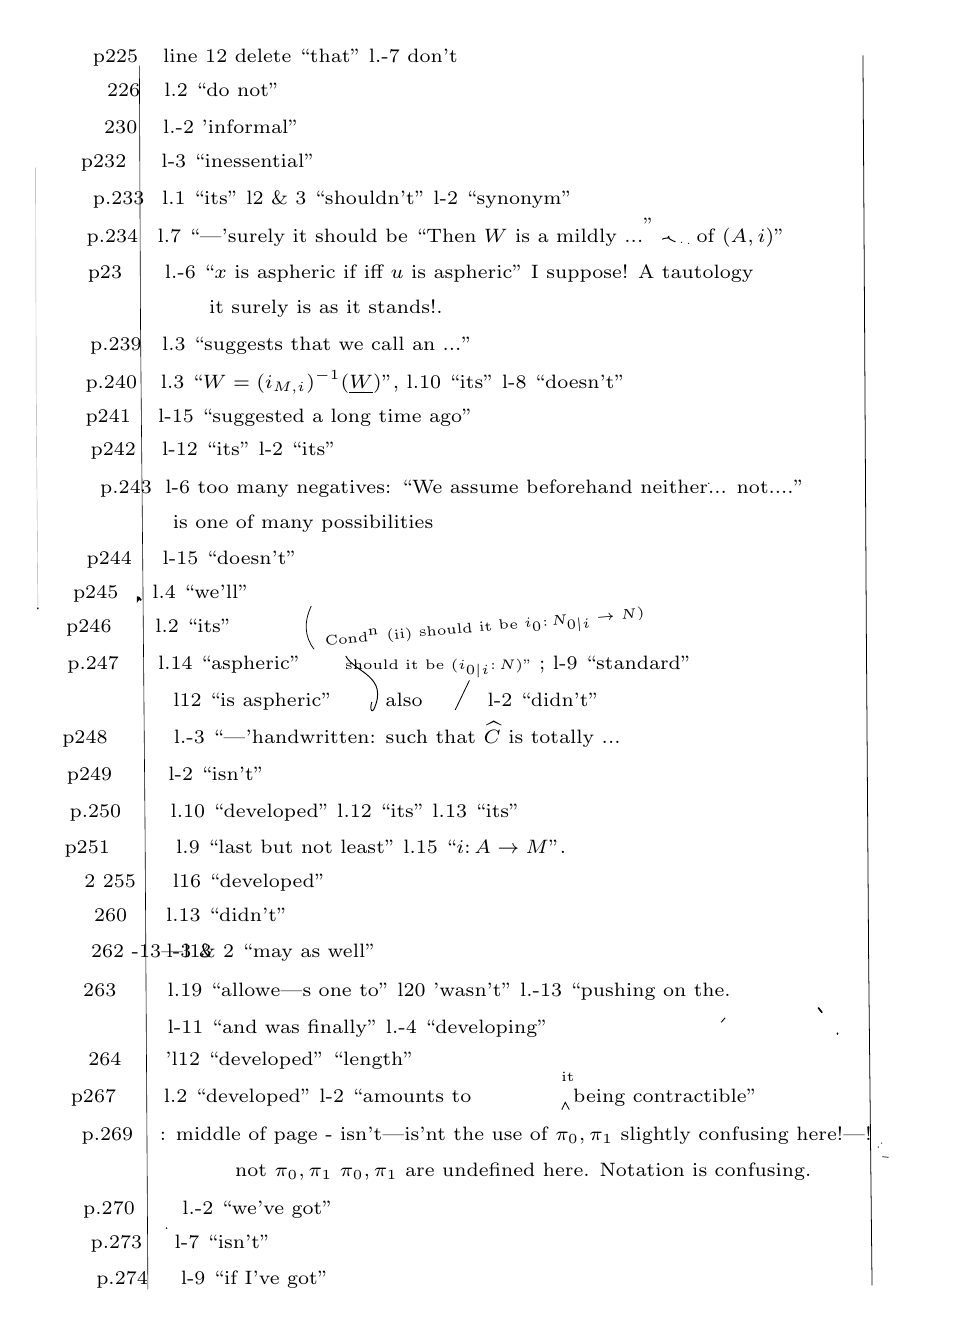
\begin{tikzpicture}[x=0.0072cm,y=-0.0072cm,every node/.style={anchor=base west,inner sep=0pt,font=\scriptsize}]
\path[use as bounding box] (35,45) rectangle (1640,2290);
% drawing-left-rule
\draw[line width=0.22pt] (232,112) -- (234,572) -- (238,1000) -- (242,1460) -- (247,2270);
% drawing-right-rule
\draw[line width=0.28pt] (1508,94) -- (1511,595) -- (1514,1120) -- (1518,1690) -- (1524,2263);
% drawing-far-left-trace: the purpose and medium of this faint trace are uncertain.
\draw[line width=0.15pt,opacity=0.35] (49,292) -- (50,685) -- (53,1065);
\fill (53,1069) ellipse [x radius=1.5,y radius=2.3];

% entry-01
\node at (149,106) {p225};
\node at (273,106) {line 12 delete ``that'' l.-7 don't};

% entry-02
\node at (174,167) {226};
\node at (275,167) {l.2 ``do not''};

% entry-03
\node at (169,231) {230};
\node at (273,231) {l.-2 'informal''};

% entry-04
\node at (128,292) {p232};
\node at (270,292) {l-3 ``inessential''};

% entry-05
\node at (149,356) {p.233};
\node at (271,356) {l.1 ``its'' l2 \& 3 ``shouldn't'' l-2 ``synonym''};

% entry-06
\node at (138,424) {p.234};
\node at (263,424) {l.7 \unsure{``|'}surely it should be ``Then $W$ is a mildly ...\raisebox{1.3ex}[0pt][0pt]{\deleted{\unsure{''}}} \tikz[baseline=-.4ex,x=.23em,y=.23em]{
  \draw[line width=.35pt] (0,0) .. controls (.6,.3) and (.9,.2) .. (1.1,.2)
    .. controls (1.2,.8) and (1.4,.6) .. (1.4,.1)
    .. controls (1.9,-.1) and (2.2,-.5) .. (2.6,-.5);
  \fill (3.8,-.6) circle (.25pt);
  \fill (5.2,-.8) circle (.22pt);
} of $(A,i)$''};

% entry-07
\node at (140,488) {\deleted{p23}};
\node at (276,488) {l.-6 ``$x$ is aspheric \deleted{\unsure{if}} iff $u$ is aspheric'' I suppose! A tautology};
\node at (354,549) {it surely is as it stands!.};

% entry-08
\node at (144,614) {p.239};
\node at (271,614) {l.3 ``suggests that we call an ...''};

% entry-09
\node at (136,681) {p.240};
\node at (269,681) {l.3 ``$W=(i_{M,i})^{-1}(\underline{W})$'', l.10 ``its'' l-8 ``doesn't''};

% entry-10
\node at (136,741) {p241};
\node at (264,741) {l-15 ``suggested a long time ago''};

% entry-11
\node at (145,799) {p242};
\node at (271,799) {l-12 ``its'' l-2 ``its''};

% entry-12
\node at (162,866) {p.243};
\node at (277,866) {l-6 too many negatives: ``We assume beforehand neither\raisebox{1.1ex}[0pt][0pt]{\makebox[0pt][l]{\tikz{\fill (0,0) circle (.25pt);}}}... not....''};
\node at (290,929) {is one of many possibilities};

% entry-13
\node at (138,992) {p244};
\node at (272,992) {l-15 ``doesn't''};

% entry-14
\node at (114,1052) {p245};
% drawing-p245-mark: the small angular mark is reproduced without assigning a punctuation function.
\draw[line width=0.6pt] (229,1048) -- (229,1055) -- (232,1051) -- (235,1055);
\node at (254,1052) {l.4 ``we'll''};

% entry-15
\node at (102,1111) {p246};
\node at (259,1111) {l.2 ``its''};

% entry-16: the written opening parenthesis of the raised insertion is drawn as the tall arc.
\node at (104,1176) {p.247};
\node at (264,1176) {\deleted{l.14 ``\unsure{aspheric}''}};
\draw[line width=0.28pt] (535,1065) .. controls (522,1093) and (523,1119) .. (540,1141);
\node[rotate=5,font=\tiny] at (559,1134) {\inserted{Cond\textsuperscript{n} (ii) should it be $i_0\colon N_{\unsure{0|i}}\to N$)}};
\node[font=\tiny] at (594,1176) {\deleted{should it be $(i_{\unsure{0|i}}\colon N\unsure{)}$\unsure{''}}};
\node at (936,1176) {; l-9 ``standard''};

% entry-17: also is physically beside the lower live correction, not before l-9.
\node at (291,1242) {l12 ``is aspheric''};
\node at (665,1242) {\inserted{also}};
\node at (845,1242) {l-2 ``didn't''};
% drawing-p247-curves: the first curve comes down from the cancelled proposal;
% the second stroke descends from the lower part of its opening parenthesis.
\draw[line width=0.35pt] (596,1153) .. controls (611,1182) and (673,1188) .. (645,1248) .. controls (641,1253) and (638,1246) .. (642,1234);
\draw[line width=0.3pt] (814,1196) -- (789,1248);

% entry-18
\node at (95,1307) {p248};
\node at (292,1307) {l.-3 \unsure{``|'}\uline{handwritten}: such that $\widehat C$ \uline{is} totally ...};

% entry-19
\node at (103,1372) {p249};
\node at (282,1372) {l-2 ``isn't''};

% entry-20
\node at (108,1437) {p.250};
\node at (286,1437) {l.10 ``developed'' l.12 ``its'' l.13 ``its''};

% entry-21
\node at (99,1501) {p251};
\node at (296,1501) {l.9 ``last but not least'' l.15 ``$i\colon A\to M$''.};

% entry-22
\node at (134,1562) {\deleted{2} 255};
\node at (290,1562) {l16 ``developed''};

% entry-23
\node at (151,1621) {260};
\node at (278,1621) {l.13 ``didn't''};

% entry-24
\node at (146,1684) {262 -\deleted{\unsure{13|l13}}};
\node at (279,1684) {l-3 \& 2 ``may as well''};

% entry-25
\node at (132,1753) {263};
\node at (281,1753) {l.19 ``allow\unsure{e|s} one to'' l20 'wasn't'' l.-13 ``pushing on the.};
\node at (281,1819) {l-11 ``and was finally'' l.-4 ``developing''};
% drawing-p263-detached-marks
\draw[line width=0.32pt] (1258,1799) -- (1265,1791);
\draw[line width=0.6pt] (1429,1773) -- (1436,1782);
\fill (1463,1819) ellipse [x radius=1.6,y radius=2.2];

% entry-26
\node at (141,1875) {264};
\node at (277,1875) {'l12 ``developed'' ``length''};

% entry-27
\node at (110,1940) {p267};
\node at (274,1940) {l.2 ``developed'' l-2 ``amounts to};
\node[font=\tiny] at (975,1904) {\inserted{it}};
\node at (996,1940) {being contractible''};
\draw[line width=.3pt] (977,1953) -- (983,1940) -- (990,1953);

% entry-28
\node at (129,2008) {p.269};
\node at (267,2008) {: middle of page - \deleted{\unsure{isn't|is'nt} the use of $\pi_0,\pi_1$ slightly confusing here}\unsure{\deleted{!}|!}};
\node at (400,2071) {\deleted{not $\pi_0,\pi_1$} $\pi_0,\pi_1$ are undefined \uline{here}. Notation is confusing.};

\fill (1535,2019) circle[radius=0.08mm];
\fill (1541,2012) circle[radius=0.08mm];
\draw[line width=0.25pt] (1542,2036) -- (1553,2037);

% entry-29
\node at (132,2138) {p.270};
\node at (307,2138) {l.-2 ``we've got''};

% entry-30
\node at (145,2197) {p.273};
% drawing-p273-point: this raised point is separate from the printed reference and the following l.
\fill (280,2162) ellipse [x radius=1.3,y radius=1.6];
\node at (293,2197) {l-7 ``isn't''};

% entry-31
\node at (155,2262) {p.274};
\node at (304,2262) {l-9 ``if I've got''};
\end{tikzpicture}%
}

% archive sheet number: 24

\scanpage{26}
% Local layout preserves the rules beside and through the correction entries.
\figure{
\begin{tikzpicture}[x=0.007cm,y=-0.007cm]
\path[use as bounding box] (80,30) rectangle (1685,2340);
% rule-left
\draw[line width=0.35pt] (233,92)--(234,830)--(237,1550)--(239,2338);
% rule-right
\draw[line width=0.35pt] (1512,86)--(1513,1018)--(1514,1700)--(1518,2225)--(1524,2338);
\draw[gray!35,line width=.25pt] (54,120) -- (53,220) -- (58,272) -- (54,335) -- (58,385) -- (54,435) -- (58,483) -- (55,516) -- (58,574) -- (54,627) -- (58,691) -- (54,745) -- (58,810) -- (55,875) -- (58,945) -- (55,1010) -- (58,1080);
% upper-left stray strokes, with no assigned textual function
\draw[gray,line width=0.15pt] (127,117).. controls (122,128) and (130,143)..(135,153);\draw[gray,line width=0.35pt] (128,116)--(125,121);\draw[gray,line width=0.35pt] (134,145).. controls (135,148) and (137,151)..(136,155);
% entry-top
\node[anchor=base west,inner sep=0pt,font=\fontsize{8}{9}\selectfont] at (265,100){l.5 commutes with. l.18 is $C\mathrel{\overset{=}{\deleted{\unsure{\Rightarrow|\to}}}}A$? confusing as it stands.};
% entry-276
\node[anchor=base east,inner sep=0pt,font=\fontsize{8}{9}\selectfont] at (220,165){276};
\node[anchor=base west,inner sep=0pt,font=\fontsize{8}{9}\selectfont] at (265,165){l.15 ``equivalent to \deleted{\unsure{``|'}}$f$\tikz[baseline]{\node[anchor=base west,inner sep=0pt] at (0,.35ex) {\inserted{\deleted{\unsure{''|'}}}};\draw[line width=.3pt] (.05em,-.65ex)--(.20em,-.15ex)--(.40em,-.65ex);} commuting with'' !};
% entry-277
\node[anchor=base east,inner sep=0pt,font=\fontsize{8}{9}\selectfont] at (220,230){277};
\node[anchor=base west,inner sep=0pt,font=\fontsize{8}{9}\selectfont] at (265,230){l.2 ``doesn't'' l-12 ``Of course''};
% entry-278
\node[anchor=base east,inner sep=0pt,font=\fontsize{8}{9}\selectfont] at (220,300){278};
\node[anchor=base west,inner sep=0pt,font=\fontsize{8}{9}\selectfont] at (265,300){l-1\tikz[baseline=(old8.base)]{\node[inner sep=0pt] (old8) {\deleted{\unsure{8}}};\node[anchor=base west,inner sep=0pt] at ([xshift=.1em,yshift=.3ex]old8.base west) {7};} \unsure{``|'}definitely'' l-8 ``isn't'' l-5 ``we'd'' (i.e we had better assume)};
% entry-279
\node[anchor=base east,inner sep=0pt,font=\fontsize{8}{9}\selectfont] at (220,360){279};
\node[anchor=base west,inner sep=0pt,font=\fontsize{8}{9}\selectfont] at (265,360){l11 ``didn't'' l-7 ``isn't''};
% entry-280
\node[anchor=base east,inner sep=0pt,font=\fontsize{8}{9}\selectfont] at (220,423){280};
\node[anchor=base west,inner sep=0pt,font=\fontsize{8}{9}\selectfont] at (265,423){l-8 ``wasn't''};
% entry-281
\node[anchor=base east,inner sep=0pt,font=\fontsize{8}{9}\selectfont] at (220,487){281};
\node[anchor=base west,inner sep=0pt,font=\fontsize{8}{9}\selectfont] at (265,487){l-11 ``which will allow us then...'' l-12 ``commutes with'' also in l-2.};
% entry-282
\node[anchor=base east,inner sep=0pt,font=\fontsize{8}{9}\selectfont] at (220,550){282};
\node[anchor=base west,inner sep=0pt,font=\fontsize{8}{9}\selectfont] at (265,550){l.5 ``commutes with''};
% entry-283a
\node[anchor=base east,inner sep=0pt,font=\fontsize{8}{9}\selectfont] at (220,612){283};
\node[anchor=base west,inner sep=0pt,font=\fontsize{8}{9}\selectfont] at (265,612){l.2 ``commutes with'' also l.17 .. l17-18 \unsure{``|'}doesn't'' + ``commutation...with''};
% entry-283b
\node[anchor=base west,inner sep=0pt,font=\fontsize{8}{9}\selectfont] at (265,676){l-1 ``commutes with''};
% entry-284
\node[anchor=base east,inner sep=0pt,font=\fontsize{8}{9}\selectfont] at (220,738){284};
\node[anchor=base west,inner sep=0pt,font=\fontsize{8}{9}\selectfont] at (265,738){l.3 ``commutation with'' l-9 ``commutes with\deleted{\unsure{''|'}}... and also with''};
% entry-285
\node[anchor=base east,inner sep=0pt,font=\fontsize{8}{9}\selectfont] at (220,803){285};
\node[anchor=base west,inner sep=0pt,font=\fontsize{8}{9}\selectfont] at (265,803){l.9. ``commutes with''};
% entry-286
\node[anchor=base east,inner sep=0pt,font=\fontsize{8}{9}\selectfont] at (220,866){286};
\node[anchor=base west,inner sep=0pt,font=\fontsize{8}{9}\selectfont] at (265,866){l15 ``its'' not ``it's'' (only used as abbrev. for ``it is''.)};
% entry-287
\node[anchor=base east,inner sep=0pt,font=\fontsize{8}{9}\selectfont] at (220,930){287};
\node[anchor=base west,inner sep=0pt,font=\fontsize{8}{9}\selectfont] at (265,930){l.17 ``structure\tikz[baseline=(su.base)]{\node[inner sep=0pt] (su) {s};\draw[line width=.45pt] ([xshift=-.5pt,yshift=-1.5pt]su.south west) -- ([yshift=-1.5pt]su.south east) -- ([yshift=-3pt]su.south east) -- ([xshift=.5pt,yshift=-3pt]su.south west) -- ([xshift=.5pt,yshift=-4.5pt]su.south west) -- ([yshift=-4.5pt]su.south east);}''};
% entry-288a
\node[anchor=base east,inner sep=0pt,font=\fontsize{8}{9}\selectfont] at (220,993){288};
\node[anchor=base west,inner sep=0pt,font=\fontsize{8}{9}\selectfont] at (265,993){l.1 ``we've got'', The phrase ``hence .... $M'$. '' \deleted{d\unsure{o|e}} has no verb.};
% entry-288b
\node[anchor=base west,inner sep=0pt,font=\fontsize{8}{9}\selectfont] at (265,1056){I suggest ``hence we have the sets etc''};
% entry-289
\node[anchor=base east,inner sep=0pt,font=\fontsize{8}{9}\selectfont] at (220,1120){289};
\node[anchor=base west,inner sep=0pt,font=\fontsize{8}{9}\selectfont] at (265,1120){l-9 ``commute with'' l-8 ``with'' not \unsure{``|'}to''};
% entry-290
\node[anchor=base east,inner sep=0pt,font=\fontsize{8}{9}\selectfont] at (220,1182){290};
\node[anchor=base west,inner sep=0pt,font=\fontsize{8}{9}\selectfont] at (265,1182){l.2 ``isn't'' l.10 ``its''};
% entry-291a
\node[anchor=base east,inner sep=0pt,font=\fontsize{8}{9}\selectfont] at (220,1246){p291};
\node[anchor=base west,inner sep=0pt,font=\fontsize{8}{9}\selectfont] at (265,1246){l.1 ``couldn't'' l.9 ``hadn't'' l.10 ``to see what \deleted{pro} stronger property};
% entry-291b
\node[anchor=base west,inner sep=0pt,font=\fontsize{8}{9}\selectfont] at (265,1308){to put in instead'' l15 'shouldn't''};
% entry-293a
\node[anchor=base east,inner sep=0pt,font=\fontsize{8}{9}\selectfont] at (220,1371){p293};
\node[anchor=base west,inner sep=0pt,font=\fontsize{8}{9}\selectfont] at (265,1371){l2. 'haven't'' l8 ``developed\tikz[baseline]{\fill[black!45] (.05em,.15ex) ellipse (.25pt and .35pt);}'' l15 ``didn't'' l-12 ``that I've got''};
% entry-293b
\node[anchor=base west,inner sep=0pt,font=\fontsize{8}{9}\selectfont] at (265,1436){l-4 ``opposite'' \deleted{l\unsure{6}}, \deleted{Replace} ``\deleted{too}\unsure{\deleted{''}|''} \deleted{by} \unsure{\deleted{``}|``}\deleted{as well}'' \deleted{for \unsure{easier reading}}.};
% entry-293c
\node[anchor=base west,inner sep=0pt,font=\fontsize{8}{9}\selectfont] at (265,1502){``too\deleted{''} in a natural way'' feels awkward. What about 'is so endowed};
% entry-293d
\node[anchor=base west,inner sep=0pt,font=\fontsize{8}{9}\selectfont] at (265,1568){in any natural way.''};
% entry-294
\node[anchor=base east,inner sep=0pt,font=\fontsize{8}{9}\selectfont] at (220,1630){p294};
\node[anchor=base west,inner sep=0pt,font=\fontsize{8}{9}\selectfont] at (265,1630){l13 ``make sense'' l-16 ``usual''};
% entry-295
\node[anchor=base east,inner sep=0pt,font=\fontsize{8}{9}\selectfont] at (220,1694){295};
\node[anchor=base west,inner sep=0pt,font=\fontsize{8}{9}\selectfont] at (265,1694){l.16 ``where'' not \raisebox{.8ex}{\unsure{``|'}}were''};
% entry-296a
\node[anchor=base east,inner sep=0pt,font=\fontsize{8}{9}\selectfont] at (220,1757){296};
\node[anchor=base west,inner sep=0pt,font=\fontsize{8}{9}\selectfont] at (265,1757){l.12 ``analogons'' isn't in the dictionary - ``analogues'' would work};
% entry-296b
\node[anchor=base west,inner sep=0pt,font=\fontsize{8}{9}\selectfont] at (265,1820){l19 ``such a functor\unsure{''|'}};
% entry-297
\node[anchor=base east,inner sep=0pt,font=\fontsize{8}{9}\selectfont] at (220,1885){p.297};
\node[anchor=base west,inner sep=0pt,font=\fontsize{8}{9}\selectfont] at (265,1885){l 1.1 ``developed''};
% entry-298
\node[anchor=base east,inner sep=0pt,font=\fontsize{8}{9}\selectfont] at (220,1950){298};
\node[anchor=base west,inner sep=0pt,font=\fontsize{8}{9}\selectfont] at (265,1950){l.3 ``standard'' l-6 ``commutes with''};
% entry-299a
\node[anchor=base east,inner sep=0pt,font=\fontsize{8}{9}\selectfont] at (220,2013){299};
\node[anchor=base west,inner sep=0pt,font=\fontsize{8}{9}\selectfont] at (265,2013){l.3 ``commute with'' \& in l.4. l.16 'developed'' l.17 ``doesn't''\tikz[baseline]{\fill (-.65em,-.8ex) circle (.35pt);\fill (-.80em,-1.2ex) circle (.32pt);}};
% entry-299b
\node[anchor=base west,inner sep=0pt,font=\fontsize{8}{9}\selectfont] at (265,2075){l20 ``its''};
% entry-300
\node[anchor=base east,inner sep=0pt,font=\fontsize{8}{9}\selectfont] at (220,2139){300};
\node[anchor=base west,inner sep=0pt,font=\fontsize{8}{9}\selectfont] at (265,2139){l.4 ``don't'' l.11 delete ``the'' l.-15 ``doesn't''};
% entry-301
\node[anchor=base east,inner sep=0pt,font=\fontsize{8}{9}\selectfont] at (220,2204){301,};
\node[anchor=base west,inner sep=0pt,font=\fontsize{8}{9}\selectfont] at (265,2204){l.-3 ``commute with''};
% entry-302
\node[anchor=base east,inner sep=0pt,font=\fontsize{8}{9}\selectfont] at (220,2270){302};
\node[anchor=base west,inner sep=0pt,font=\fontsize{8}{9}\selectfont] at (265,2270){l.1. 'commute with \deleted{\unsure{''|'}} finite products and with'' l.5 ``commutation with''};
\end{tikzpicture}
}
% archive sheet number: 25

\scanpage{27}
\begingroup
\setlength{\parindent}{0pt}
\everypar{\hangindent=2.9em\hangafter=1}
\noindent\tikz[remember picture,overlay]{\coordinate (ruleA27top);}

\unsure{302} l.\unsure{15} ``its

303 l.1 ``\deleted{\unsure{with|who}} which will be'' l2 ``we've got'' l.-3 ``image of $A$ by $A$'' - not clear what you mean.

304 l-15 ``commutes with'' also l-13. \deleted{\unsure{l-2} ``play'' \unsure{no|not} ``s}\unsure{\deleted{''}|''}

305 l.5 ``interpret' l14 ``commutes with''

306 l.19 ``its'' \deleted{l} also l-5. l-4 ``test \uline{category}''

309 l.-8 ``on \uline{the} previous''

312 l-.8 ``isn't'' \deleted{l-6 \unsure{lets|let's}}

313 l9 ``shouldn't'' l.18 ``don't'' l-12 ``commutes with''

\noindent\hspace*{2.9em}\deleted{filtering} \raisebox{1.1ex}[0pt][0pt]{\unsure{\deleted{\unsure{out|at|on|or}}|\unsure{out|at|on|or}}} \unsure{\deleted{l-2}|l-2|\deleted{l-7}|l-7} filtering''

314 l.5 ``isn't'' l.6 ``as is''

315 Sent\tikz[baseline=(sentA27.base)]{\node[inner sep=0pt] (sentA27) {\deleted{\unsure{ann|en}}};\node[anchor=base west,inner sep=0pt] at (sentA27.base west) {en};}ce starting l.7 - difficult to understand. Possibly: 'I add this comment, of course, \deleted{to} in order to ``\uline{push home}'' the point that \uline{no more} with resp... than in any other essential \tikz[baseline=(respectA27.base)]{\node[inner sep=0pt] (respectA27) {respect.};\draw[line width=.65pt,line cap=round] ([xshift=1.2em,yshift=-.55ex]respectA27.base west) -- ++(.12em,-.13ex);} concerning the ability \uline{to express} basic situations.....theory, \uline{does} the cat. ... \uline{stand} singled out. \deleted{(This is \raisebox{1.2ex}[0pt][0pt]{\makebox[0pt][l]{\inserted{certainly}}} true \tikz[baseline=(presA27.base)]{\node[inner sep=0pt] (presA27) {\unsure{presumably}};\node[anchor=base west,inner sep=0pt] at ([yshift=1.3ex]presA27.base west) {\inserted{as far as our}};} at the present knowledge goes). \tikz[baseline=(noA27.base)]{\node[inner sep=0pt] (noA27) {\unsure{No|Now}};\fill ([xshift=.15em,yshift=-.45ex]noA27.base west) circle (.3pt);}- -}. (This certainly seems to be so as far as our present knowledge goes\tikz[baseline=0pt,x=1ex,y=1ex]{\fill (.07,.22) circle (.025);\draw[line width=.5pt] (.22,.45)--(.42,.51);})''...

\noindent\hspace*{2.9em}l.17 ``\tikz[baseline=(root27its.base)]{\node[inner sep=0pt] (root27its) {its};\draw[line width=.35pt,line cap=round] ([xshift=.01em,yshift=1.65ex]root27its.base west)--++(.05em,-.08ex)--++(-.01em,-.07ex);}'' l.-3 'and which \tikz[baseline=0pt,x=1ex,y=1ex]{\draw[line width=.55pt] (0,-1.05)--(.15,-.45)--(.3,-1.02);}\raisebox{1.3ex}[0pt][0pt]{\makebox[0pt][l]{\inserted{would}}} allow one to compute''\tikz[remember picture,overlay]{\coordinate (ruleA27gap) at (0,-2.1ex);}

\noindent\hspace*{3em}\tikz[baseline=0pt,x=1ex,y=1ex]{\draw[line width=.55pt,line cap=round] (0,0)--(.23,.07);}\par

\noindent\tikz[remember picture,overlay]{\coordinate (ruleA27restart) at (0,1.7ex);}316. l.1 ``shouldn't'' l12 ``$i(a)$ \deleted{it} is a ''\deleted{\unsure{to|is}}

317. l.11 ``its'' l-16 ``isn't''

320 l 8. ``indispensable'' l-15 'developing'' l-8 ``its''

321 l.9 'isn't''

323 l13 ``don't''

326 l-12 \deleted{\unsure{\&|l}}\tikz[baseline=0pt,x=1ex,y=1ex]{\fill (.1,-.32) circle (.035);} \& l.-8 \tikz[baseline=(B27comm.base),x=1em,y=1ex]{
  \node[anchor=base west,inner sep=0pt] (B27comm) at (0,0) {``commutes \uline{with}''};
  \node[anchor=base west,inner sep=0pt] at (-.55,2.1) {\inserted{\& l-3}};
  \fill (2.55,3.0) circle (.035em);
  \draw[line width=.4pt] (-.28,.9)--(-.55,-1.9);
  \draw[line width=.4pt] (-.47,-1.1)--(-.35,-1.45)--(-.25,-1.1);
} and

p.327. l7 ``$\alpha:\mathord{\tikz[baseline=0pt,x=1ex,y=1ex]{\draw[line width=.085ex,line cap=round,line join=round] (.19,0)--(.86,1.37)--(1.08,0)--(.71,.025) (.61,.032)--(.19,0) (-.05,.08)--(.51,1.12);}}\longrightarrow \mathord{\tikz[baseline=0pt,x=1ex,y=1ex]{\draw[line width=.085ex,line cap=round,line join=round] (.20,0)--(.83,1.12)--(1.22,.05)--(.82,.04) (.72,.02)--(0,0)--(.64,.99);}}/F$'' should it be '

\noindent\hspace*{2.9em}l-17 ``allows \uline{one} to'' l-16 ``doesn't'' l-14 ``isn't\deleted{\unsure{''|'}} there!''

\noindent\hspace*{2.9em}l-5 ``don't''

p328 l-12 \deleted{would'nt} should ``wouldn't'' = ``shouldn't''

\noindent\hspace*{2.9em}l-10 doesn't

p329 l.6 $\mathord{\tikz[baseline=0pt,x=1ex,y=1ex]{\draw[line width=.09ex,line cap=round,line join=round] (.16,-.05)--(.77,1.5)--(1.21,.04)--(.16,.0) (.49,1.36)--(-.04,0)--(.21,0);}}$ (doubled side is missing) ``its''

\noindent\hspace*{2.9em}l12 \unsure{``|'}don't'' l-13 ``makes sense'' l.-13 \unsure{``|'}semisimplicial\unsure{,|.} \tikz[baseline=0pt,x=1ex,y=1ex]{\draw (0,-.6)--(.45,1.7); \draw (.14,.1)--(.43,-.1);}\tikz[baseline=0pt,overlay,x=1em,y=1ex]{\fill (1.0,5.3) circle (.035em);\fill (.84,4.9) circle (.035em);}\raisebox{1.9ex}[0pt][0pt]{\inserted{l-5\tikz[baseline=0pt,x=1ex,y=1ex]{\fill (.08,.08) circle (.04);} ``enveloping\unsure{'|''}}} \margin{
\begin{tikzpicture}[x=1em,y=1ex,baseline=(margA27.base)]\node[anchor=base west,inner sep=0pt] at (.8,2.1) {?};\begin{scope}[rotate=14]\node[anchor=base west,inner sep=0pt] (margA27) at (0,0) {I'm not certa};\node[anchor=base west,inner sep=0pt] at (-.1,-1.8) {if it is 1 or 2 p};\draw[line width=.45pt] (-.65,-.55) .. controls (-1.15,-2.5) and (-.25,-3.0) .. (1.3,-2.8);\end{scope}\fill (3.8,-3.3) circle (.035em);\end{tikzpicture}}
% slanted; right edge of the note is clipped

p.333 l.-12 ``makes sense''

p.334 l.3 '$b\in A_{n-1}$'' l-6 ``its'' also in l-5.
\tikz[remember picture,overlay]{\coordinate (ruleA27bottom) at (0,-3ex);
% left rule, two observed segments with a small break above 316
\draw[line width=.35pt] ([xshift=1.9em,yshift=1.3ex]ruleA27top)--([xshift=1.9em]ruleA27top |- ruleA27gap);
\draw[line width=.35pt] ([xshift=1.9em]ruleA27top |- ruleA27restart)--([xshift=1.9em]ruleA27top |- ruleA27bottom);
% right rule, beside and sometimes through the end of long text lines
\draw[line width=.4pt] ([xshift=\linewidth,yshift=1.3ex]ruleA27top)--([xshift=\linewidth]ruleA27top |- ruleA27bottom);
}
\endgroup

% archive sheet number: 26

\scanpage{28}

% The list and the ruled sheet share one coordinate field. Coordinates reproduce
% the supplied image's relative positions, including the long blank lower part.
% The faint far-left trace has fading, indeterminate ends: the path represents
% the observed segment, not an asserted original endpoint or a named operation.
\noindent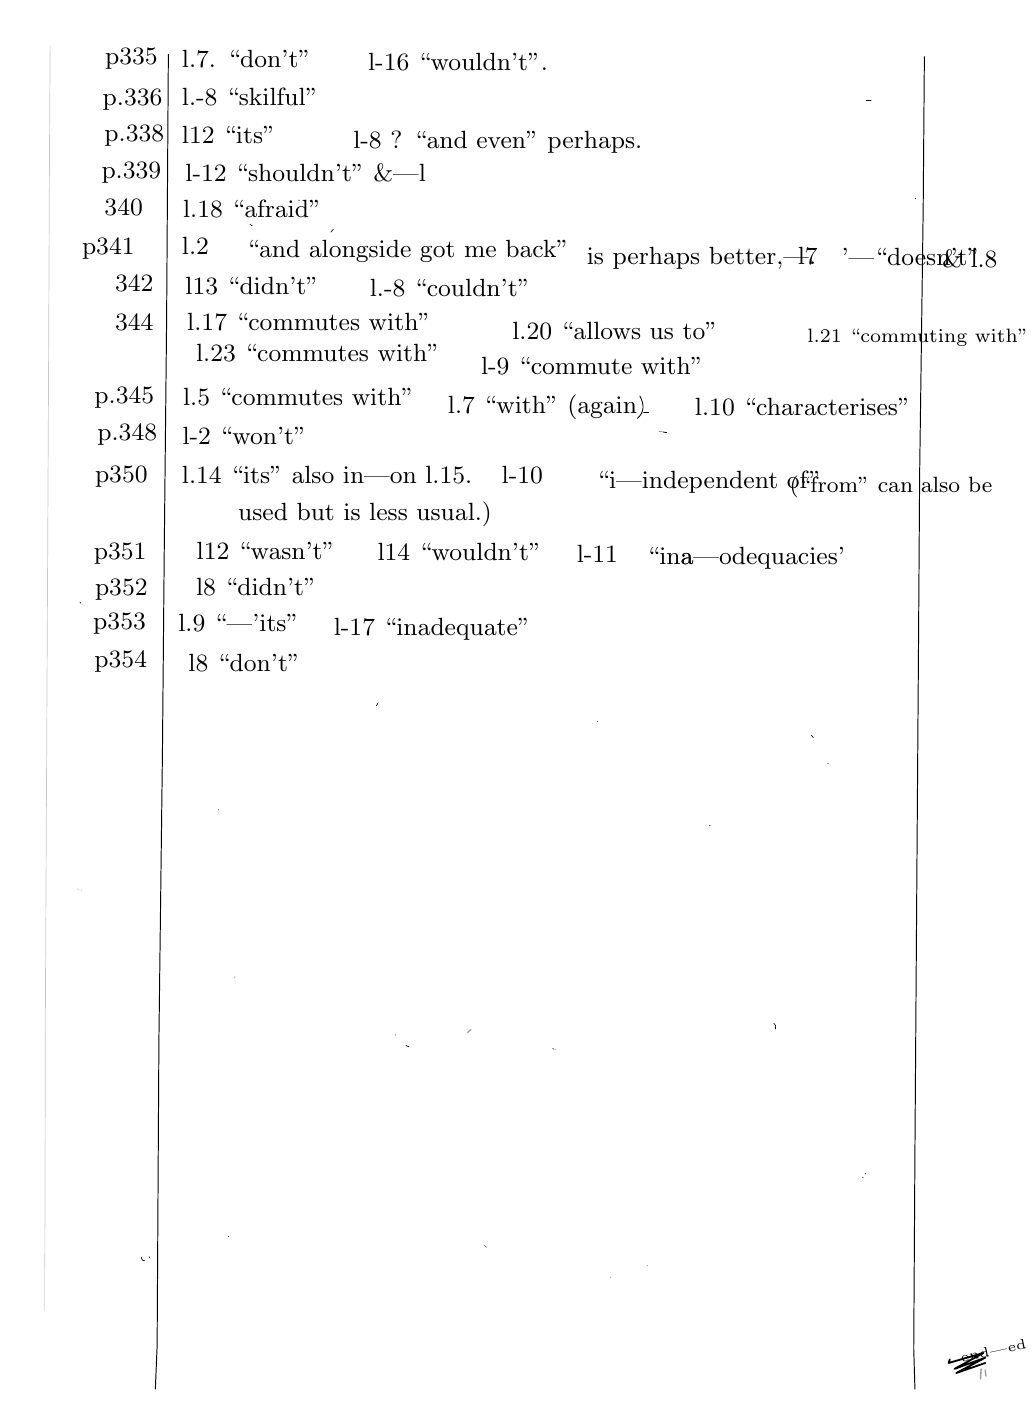
\begin{tikzpicture}[x=.0075cm,y=-.0075cm,line cap=round,line join=round]
\path[use as bounding box] (20,45) rectangle (1670,2348);
% BEGIN left_rule
\draw[line width=.35pt] (258,90)--(255,545)--(251,935)--(248,1270)--(242,1760)--(239,2275)--(236,2348);
% END left_rule
% BEGIN right_rule
\draw[line width=.35pt] (1537,94)--(1535,350)--(1529,800)--(1527,1100)--(1524,1520)--(1521,1950)--(1519,2280)--(1521,2348);
% END right_rule
% BEGIN faint_trace
\draw[black!22,line width=.25pt] (58,75)--(57,240)--(55,700)--(53,1100)--(50,1700)--(49,2140);\draw[black!12,line width=.25pt] (49,2140)--(49,2215);
% END faint_trace
% Prominent isolated marks, with no assigned punctuation or editorial function.
% BEGIN upper_right_dash
\draw[line width=.18pt] (1439,168)--(1447,168);
% END upper_right_dash
% BEGIN right_point
\fill (1522,334) circle[radius=1.0];
% END right_point
% BEGIN afraid_marks
\fill (479,337) circle[radius=1.1];\draw[line width=.24pt] (396,378)--(400,380);\draw[line width=.24pt] (533,391)--(537,386);
% END afraid_marks
% BEGIN again_mark
\draw[black!40,line width=.3pt] (1088,728)--(1093,728);
\draw[line width=.3pt] (1095,729)--(1101,730);
% END again_mark
% BEGIN left_352_point
\fill (109,1018) circle[radius=1.1];
% END left_352_point
% BEGIN lower_left_marks
\draw[line width=.24pt] (212,2125)--(214,2130)--(218,2131);\fill (226,2125) circle[radius=1.1];
% END lower_left_marks
% BEGIN lower_right_marks
\fill (1433,1990) circle[radius=1.0];\fill (1437,1984) circle[radius=1.0];
% END lower_right_marks

\begin{scope}[every node/.style={anchor=base west,inner sep=0pt,font=\fontsize{9}{11}\selectfont}]
\node at (150,108) {p335};
\node at (280,113) {l.7. ``don't''};
\node at (595,118) {l-16 ``wouldn't''.};

\node at (146,176) {p.336};
\node at (280,177) {l.-8 ``skilful''};

\node at (149,237) {p.338};
\node at (280,241) {l12 ``its''};
\node at (570,249) {l-8 ? ``and even'' perhaps.};

\node at (144,301) {p.339};
\node at (286,305) {l-12 ``shouldn't'' \deleted{\unsure{\&|l}}};

\node at (149,363) {340};
\node at (282,366) {l.18 ``afraid''};

\node at (111,429) {p341};
\node at (280,429) {l.2};
\node at (389,434) {``and alongside \uline{got me} back''};
\node at (965,445) {is perhaps better\unsure{,|.}};
\node at (1322,445) {l7};
\node at (1396,448) {\unsure{'|``}doesn't''};
\node at (1566,450) {\& l.8};

\node at (167,491) {342};
\node at (286,496) {l13 ``didn't''};
\node at (598,499) {l.-8 ``couldn't''};

\node at (167,557) {344};
\node at (289,558) {l.17 ``commutes with''};
\node at (839,573) {l.20 ``allows us to''};
\node[font=\fontsize{7}{9}\selectfont] at (1338,578) {l.21 ``commuting with''};

\node at (304,610) {l.23 ``commutes with''};
\node at (786,631) {l-9 ``commute with''};

\node at (132,680) {p.345};
\node at (282,685) {l.5 ``commutes with''};
\node at (730,697) {l.7 ``with'' (again\tikz[baseline=0pt,x=1ex,y=1ex]{\draw[line width=.08ex,line cap=round] (.10,1.6) .. controls (.53,.8) and (.52,.05) .. (-.12,-.48);\draw[line width=.08ex,line cap=round] (.46,.04)--(.92,.04);}};
\node at (1148,701) {l.10 ``characterises''};

\node at (137,744) {p.348};
\node at (281,750) {l-2 ``won't''};

\node at (133,815) {p350};
\node at (280,817) {l.14 ``its'' also \unsure{in|on} l.15.};
\node at (821,817) {l-10};
\node at (981,824) {``\unsure{\uuline{i}|\uline{i}}ndependent of''};
\node[font=\fontsize{8}{10}\selectfont] at (1308,831) {(``from'' can also be};
\node at (375,879) {used but is less usual.)};

\node at (131,944) {p351};
\node at (305,944) {l12 ``wasn't''};
\node at (611,947) {l14 ``wouldn't''};
\node at (948,950) {l-11};
\node at (1066,953) {``in\tikz[baseline=(aold28A.base)]{\node[inner sep=0pt] (aold28A) {\deleted{\unsure{a|o}}};\node[anchor=base west,inner sep=0pt] at (aold28A.base west) {a};}dequacies'};

\node at (133,1006) {p352};
\node at (304,1005) {l8 ``didn't''};

\node at (130,1063) {p353};
\node at (274,1066) {l.9 \unsure{``|'}its''};
\node at (537,1073) {l-17 ``inadequate''};

\node at (132,1127) {p354};
\node at (291,1134) {l8 ``don't''};
\end{scope}

% The cancelled marginal word is at the foot of the sheet, outside the right
% rule. The cancellation traverses the whole word; its buried n is not secure.
% Isolated lower-field marks: shape only, physical origin unassigned.
% blank_slash_01
\draw[line width=.22pt,line cap=round] (610,1192)--(613,1187);
% blank_point_02
\fill[black!70] (984,1219) circle[radius=.9];
% blank_slash_03
\draw[line width=.23pt,line cap=round] (1346,1242)--(1349,1246);
% blank_point_04
\fill (1374,1290) circle[radius=1.0];
% blank_point_05
\fill[black!65] (343,1368) circle[radius=.8];
% blank_point_06
\fill (1174,1395) circle[radius=1.05];
% blank_faint_dash_07
\fill[black!40] (104,1502) ellipse[x radius=.6,y radius=.8];\fill[black!35] (107,1503) ellipse[x radius=.6,y radius=.7];\fill[black!40] (111,1505) ellipse[x radius=.7,y radius=.5];
% blank_faint_curve_08
\draw[black!40,line width=.16pt] (369,1653)--(371,1650);
% blank_curve_09
\draw[line width=.23pt] (1282,1729)..controls(1286,1731)and(1286,1735)..(1285,1739);
% blank_gray_mark_10
\draw[black!35,line width=.48pt,line cap=round] (764,1745)--(770,1740);
% blank_point_11
\fill[black!75] (642,1749) circle[radius=.9];
% blank_mark_12
\draw[line width=.27pt,line cap=round] (660,1767)--(665,1769);
% blank_dash_13
\draw[line width=.20pt] (908,1772)--(910,1773);\draw[black!30,line width=.16pt] (910,1773)--(914,1774);
% blank_point_15
\fill (360,2090) circle[radius=.95];
% blank_mark_16
\draw[black!70,line width=.22pt] (793,2105)--(796,2108);
% blank_point_18
\fill[black!65] (1068,2139) circle[radius=.8];
% blank_point_19
\fill[black!65] (1006,2159) circle[radius=.8];
% BEGIN bottom_note
\node[rotate=12,font=\tiny,anchor=base west] (end28C) at (1584,2306) {\deleted{\unsure{end|ed}}};
\draw[line width=.65pt,line cap=round,line join=round] (1580,2298)--(1578,2304)--(1637,2287)--(1588,2314)--(1640,2295)--(1591,2321)--(1640,2304);
\draw[black!40,line width=.5pt] (1633,2314)--(1632,2331) (1640,2316)--(1641,2326);
% END bottom_note
\end{tikzpicture}

% archive sheet number: 27

\scanpage{29}

% The orange-black feature above-left of p335 is a material blemish, not a quotation stroke.
% Two pale vertical traces are interpreted as paper creases; see the layout report.
p335 l.7. ``don't'' l-16 ``wouldn't''

% Two separate small dark points in the left margin, physical origin unassigned.
\noindent\tikz[overlay,x=1ex,y=1ex]{\fill (-1.1,.95) circle (.045);\fill (-.91,.79) circle (.035);}p.336 l.-8 ``skilful''\margin{\begin{tikzpicture}[x=1ex,y=1ex]\draw[gray,line width=.10ex,line cap=round] (.2,0) .. controls (.08,.24) and (.12,.45) .. (.18,.65);\draw[gray!55,line width=.08ex] (.46,.95)--(.60,1.06);\draw[gray!45,line width=.06ex] (.75,1.28)--(.74,1.41);\end{tikzpicture}}
% The short right-margin stroke is below the archive number; no letter value assigned.

p.338 l12 ``its'' l-8 ? ``and even'' \tikz[baseline=(perhaps29.base)]{\node[inner sep=0pt] (perhaps29) {perhaps};\fill[black!45] ([xshift=1.55em,yshift=-1.0ex]perhaps29.base east) circle (.045ex);}

p.339 l-12 ``shouldn't'' \deleted{\unsure{\&|l}}

340 l.18 ``afraid''

p341 l.2 ``and alongside \uline{got me} back'' is perhaps better\unsure{,|.} l7 \unsure{'|``}doesn't'' \& l.8

342 l13 ``didn't'' l.-8 ``couldn't''

344 l.17 ``commutes with'' l.20 ``allows us to'' l.21 ``commuting with''

l.23 ``commutes with'' l-9 ``commute with''

p.345 l.5 ``commutes with'' l.7 ``with'' (again\tikz[baseline=0pt,x=1ex,y=1ex]{\draw[line width=.08ex,line cap=round] (.10,1.6) .. controls (.53,.8) and (.52,.05) .. (-.12,-.48);\draw[line width=.08ex,line cap=round] (.46,.04)--(.92,.04);} l.10 ``characterises''

p.348 l-2 ``won't''

p350 l.14 ``its'' also \unsure{in|on} l.15. l-10 \unsure{``|'}\unsure{\uuline{i}|\uline{i}}ndependent of'' (``from'' can also be used but is less usual.)

p351 l12 ``wasn't'' l14 ``wouldn't'' l-11 ``in\tikz[baseline=(old29C.base)]{\node[inner sep=0pt] (old29C) {\deleted{\unsure{a|o}}};\node[anchor=base west,inner sep=0pt] at (old29C.base west) {a};}dequacies'

p.352 l8 ``didn't''

p353 l.9 \unsure{``|'}its'' l-17 ``inadequate''

p354 l8 ``don't''

Sent 6/2/84

\figure{
\begin{tikzpicture}[x=.92\linewidth,y=1ex]\draw (0,.2) .. controls (.15,1.2) and (.32,-.8) .. (.49,-.35) .. controls (.67,.35) and (.85,.25) .. (1,.05);\end{tikzpicture}}

p354 l.-10 ``didn't'', l-11 ``isn't'' l-3 ``its''

p.355 l.-4 ``which'' l-3 do you mean \unsure{``|'}from $(*)$''

p356 l1 ``isn't'' (indistinct in my copy) l6 ``we've got'', \deleted{\unsure{Formulae|Formulæ} $(2)$ and $(B)$ are unreadable. Are they} l.-2 ``we've got''

p357 l.1 ``we've got'' \deleted{$(2)\quad f^{*}(\unsure{\beta|g|S}_{\unsure{M|m}})\unsure{=|-}\unsure{?|s}$} l-17 ``commutes with''

p358 l.1. ``didn't'' l.4 ``shouldn't'' l8 ``don't'' l.9 \unsure{``|'}been wasting my time''

% An isolated point stands over the first part of commutes; no punctuation role assigned.
l-4 \unsure{``|'}\tikz[baseline=(cm29C.base)]{\node[inner sep=0pt] (cm29C) {commutes};\fill ([xshift=-.65em,yshift=.9ex]cm29C.north) circle (.035ex);} with''

p359 l16 'its''

% Four distinct points around and above l are preserved without assigning a punctuation value.
p360 \tikz[baseline=(l360C.base)]{\node[inner sep=0pt] (l360C) {l};\fill ([xshift=.2em,yshift=1.5ex]l360C.north east) circle (.055ex);\fill ([xshift=.12em,yshift=.92ex]l360C.north east) circle (.055ex);\fill ([xshift=.95em,yshift=.6ex]l360C.north east) circle (.035ex);\fill ([xshift=.02em,yshift=-.08ex]l360C.north east) circle (.045ex);}-17 \tikz[baseline=(quote360C.base)]{\node[inner sep=0pt] (quote360C) {``};\fill ([yshift=-.35ex]quote360C.south) circle (.03ex);}\unsure{than|then} looking'' .. l-16 ``and trying'' l-5 ``didn't''
% One separate low point is below the opening quote before than/then.

p361 l16 \unsure{'|``}didn't''

p362 l.7 \unsure{'|``}interpret''

p363 l-8 ``shouldn't''\margin{\tikz[x=1ex,y=1ex]{\fill (0,0) circle (.045);\fill (.2,.28) circle (.045);}}
% Two detached points in the right margin, with physical origin unassigned.

p365 l.4 ``its'' l-19 \unsure{``|'}isn't'' l-17 ``isn't'' l-4 'doesn't''

p367 l-13, ``its''

p369 l.4, \unsure{'|``}suggests that one views'' l-13 ``its'' l-5 ``didn't'' l-4 ``don't''

p370 l6 ``its'' also l.-3.

p371 l14 ``its'' l18 ``don't'' l20 ``in which I was working'' l.21 ``wasn't''

\margin{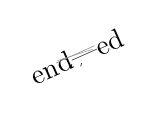
\begin{tikzpicture}[x=1ex,y=1ex]
\node[rotate=24,inner sep=0pt] (end29) at (0,0) {\deleted{\unsure{end|ed}}};
\draw[black!45,line width=.22pt] (-1.7,-.55)--(1.5,.90);
\draw[black!40,line width=.20pt] (-1.6,-.35)--(1.35,.60);
\draw[line width=.22pt] (-.45,-.95)--(-.40,-.65);
\draw[line width=.22pt] (.35,-.82)--(.42,-.57);
\end{tikzpicture}}
% The pale cancelled marginal cluster meets the lower sheet edge; no additional letters are supplied.

% archive sheet number: 28

\scanpage{30}
% Pale near-vertical strips and the rimmed lower-right spot are material features.
% Isolated dark marks are reproduced without assigning a writer or textual function.

p. 371 l\unsure{-|.}14 ``\tikz[baseline=(did30C.base)]{\node[inner sep=0pt] (did30C) {didn't};\begin{scope}[shift={(did30C.base west)},x=1em,y=1ex]\draw[overlay,black!45,line width=.3pt,line cap=round] (-1.05,.55) .. controls (-1.1,.18) and (-.93,.15) .. (-.8,.15) -- (-.1,.08);\draw[overlay,black!45,line width=.3pt,line cap=round] (-.55,.6) .. controls (-.65,.15) and (-.46,.04) .. (-.45,-.28);\end{scope}}''

p 372 l 1.6 ``commutes with'' \quad l.17 ``with small \ldots{} and finite \unsure{unverse|inverse|universe}''

l.21 ``commute with'' \quad l-12 ``commute with'' \quad l-5 ``its''

p 373 l-13 \unsure{``|`}recommendation''

p.373 l 2 ``its''. \quad line 3 of 101 ``no question of dealing'' \quad \S101 l.11 ``commuting with'' \quad l-6 ``its''

p.374 l 10 ``commutation :.. with''

p 377 l.-\tikz[baseline=(ref377.base)]{\node[inner sep=0pt] (ref377) {15};\fill[overlay,black!65] ([xshift=.53em,yshift=.60ex]ref377.base west) circle (.035ex);} ``its'' \quad l-7 ``won't'' \quad l-3 `don't'' \tikz[overlay,x=1em,y=1ex]{\fill (7.0,.25) ellipse (.025 and .055);}

378 l-7 ``interpret'' \quad l-1 ``commuting with''

379 l 1 not ``to'' ``\uuline{with}'' \quad l 8 ``made up of'' \quad ``commute with''

l.15 ``insufficient''

p 380 l.15 ``don't\unsure{'|''}

p-381 l\unsure{-|.}\tikz[baseline=(old381C.base)]{\node[inner sep=0pt] (old381C) {\deleted{\unsure{8}}};\node[anchor=base west,inner sep=0pt] at (old381C.base west) {3};} ``commuting with''

p 382 l.1 ``haven't'' \quad l 3 ``hadn't'' \quad l.5 ``breathe''

l.7 `covered'' (typing slip.) \quad l 14 ``out to prove''

p 383 l.10 ``inaccurate'' \quad l 11 ``its'' \quad l -10 `doesn't'' \quad l-9 ``much sense in bothering\unsure{''|'} \quad l-8 ``invaluable'' \quad l-3 \unsure{``|`}suggest simply dropping''

p 384 l 8 ``made up of''

p 385 l 6 ``commutes with \ldots{} (resp. with....)'' \quad l-14 ``symmetrically''

Formula (7) \unsure{\raisebox{1.1ex}[0pt][0pt]{$+$}|``|`}$\cong$'' missing

386 l.-11 ``as \uline{is} well known too'' \quad l-6 ``without''

p 387 l-17 ``commute\deleted{\unsure{s}} with'' \quad l.-3 `commuting with''

p 388 l 13 ``equivalent \deleted{with}'' to'' is more usual\unsure{,|.}

p 390 l 16 ``interpret''

p 392 l 8 ``its'' \quad l-1 ``afraid''

p 393 l-10 ``didn't''\tikz[overlay,x=1em,y=1ex]{\fill[black!65] (11.5,1.8) circle (.035);}\tikz[overlay,x=1em,y=1ex]{\draw[black!55,line width=.25pt,line cap=round] (14.7,.85)--(14.75,.60);}

p 394 l-7 \tikz[baseline=(with394C.base)]{\node[inner sep=0pt] (with394C) {``commutes with''};\fill ([xshift=2.8em,yshift=1.0ex]with394C.base east) ellipse (.045ex and .09ex);}

p 395 l 1 \unsure{``|`}interpreted as saying\unsure{''|'} is more usual. \quad l 4 ``commute with''

l 16 ``interpret''

p 396 l.-4 ``commute with'' again l-2. \margin{\tikz[x=1ex,y=1ex]{\fill (0,0) circle (.055);\fill (.23,.29) -- (.22,.40) -- (.34,.34) -- (.30,.28) -- cycle;}}

p.39\unsure{7|1} l-13 ``its'' also in l-12

p.399 l 6 ``commutes with'' \quad l 17 ``analogue'' \quad l 19 ``its''

p 400 l-8 ``developed''

p 401 l.7 ``didn't''. \quad l.-11 \unsure{`|``}\tikz[baseline=(km401C.base)]{\node[inner sep=0pt] (km401C) {$(k-M)$};\fill[overlay] ([xshift=-.3em,yshift=1.1ex]km401C.base west) circle (.055ex);}''
% archive sheet number: 23 (possibly 29)

\scanpage{31}
% One handwritten correction list. Two vertical traces are preserved geometrically;
% their ink/material origin is unassigned. Circular edge impressions are material.
\noindent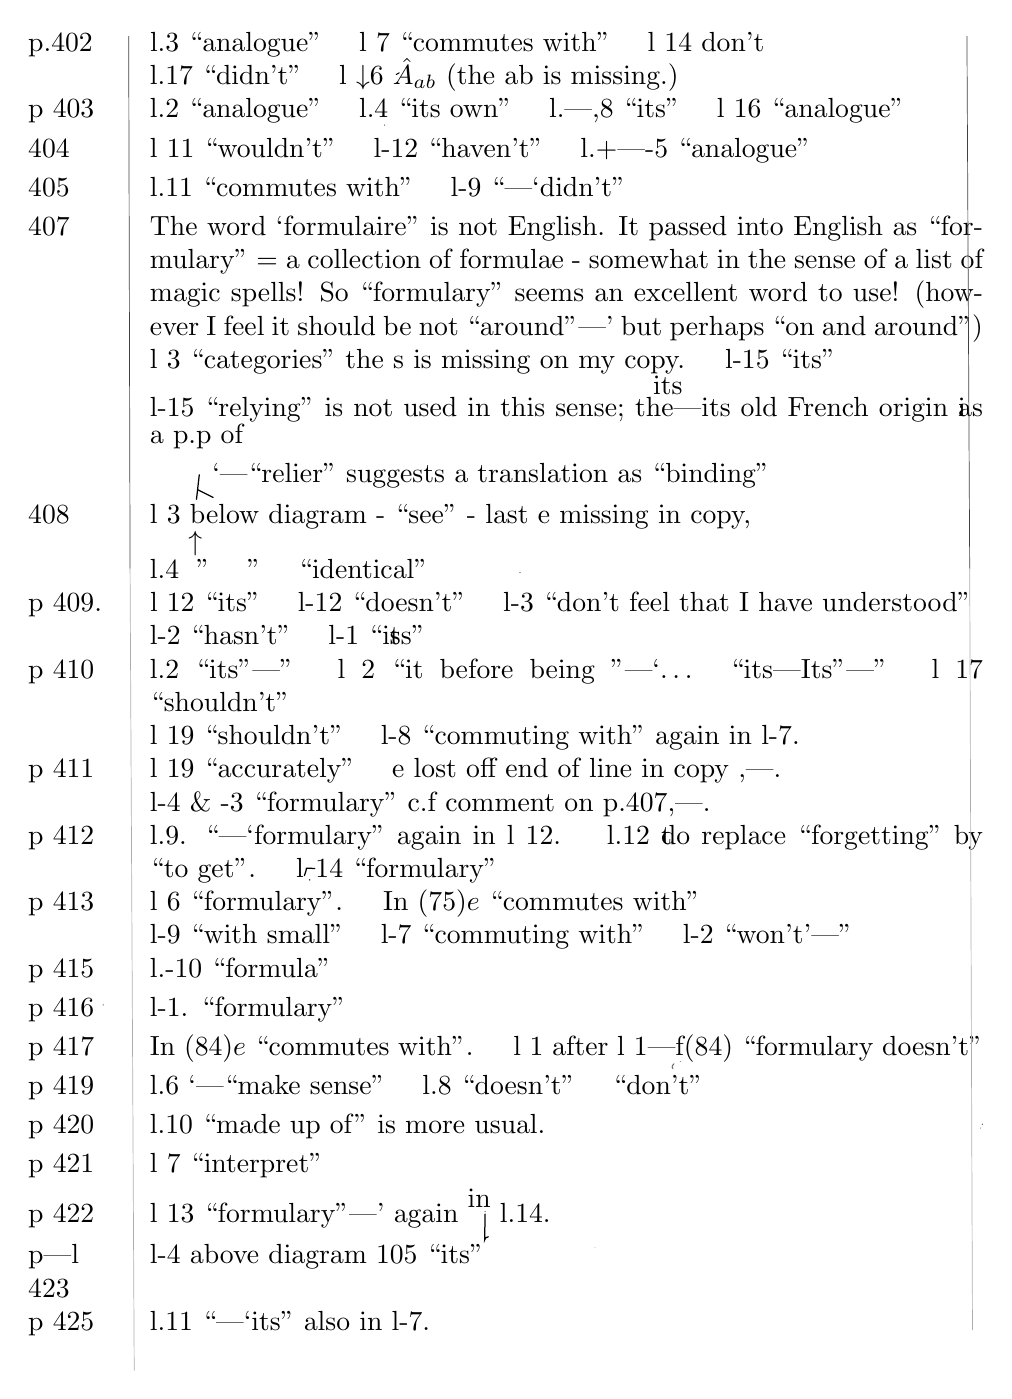
\begin{tikzpicture}
\node[anchor=north west,inner sep=0pt] (sheet031B) {%
\begin{minipage}{\linewidth}
\begin{tabular}{@{}p{3.4em}@{\hspace{1em}}p{\dimexpr\linewidth-4.4em\relax}@{}}
p.402 & l.3 ``analogue'' \quad l 7 ``commutes with'' \quad l 14 don't\par l.17 ``didn't'' \quad l $\downarrow$6 \tikz[baseline=(hat031.base)]{\node[inner sep=0pt] (hat031) {$\hat{A}_{ab}$};\draw[overlay,line width=.35pt,line cap=round] ([xshift=.14em,yshift=.85ex]hat031.base west)--([xshift=.25em,yshift=1.0ex]hat031.base west);} (the ab is missing.) \\[.5ex]

p 403 & l.2 ``analogue'' \quad \tikz[baseline=(ref403B.base)]{\node[inner sep=0pt] (ref403B) {l.4};\fill ([xshift=-.15em,yshift=-.6ex]ref403B.base east) circle (.045ex);} ``its \deleted{own}'' \quad l\unsure{.|,}8 ``its'' \quad l 16 ``analogue'' \\[.5ex]

404 & l 11 ``wouldn't'' \quad l-12 ``haven't'' \quad l.\unsure{+|-}5 ``analogue'' \\[.5ex]

405 & l.11 ``commutes with'' \quad l-9 \unsure{``|`}didn't'' \\[.5ex]

407 & The word `formulaire'' is not English. It passed into English as ``formulary'' $=$ a collection of formulae - somewhat in the sense of a list of magic spells! So ``formulary'' seems an excellent word to use! (however I feel it should be not ``around\unsure{''|'} but perhaps ``on and around'')\par l 3 ``categorie\uline{s}'' the s is missing on my copy. \quad l-15 ``its''\par l-15 ``relying'' is not used in this sense; \tikz[baseline=(old407B.base)]{\node[inner sep=0pt] (old407B) {\deleted{\unsure{the|its}}};\node[anchor=south west,inner sep=0pt] at ([xshift=.65em,yshift=.1ex]old407B.north west) {\inserted{its}};} old French origin \tikz[baseline=(as407B.base)]{\node[inner sep=0pt] (as407B) {\deleted{\unsure{i}}};\node[anchor=base west,inner sep=0pt] at (as407B.base west) {a};}s \tikz[baseline=(rel407C.base)]{\node[inner sep=0pt] (rel407C) {\unsure{`|``}relier''};\node[anchor=south,inner sep=0pt] at ([xshift=-.55em,yshift=1.1ex]rel407C.north west) {\inserted{a p.p of}};\draw[line width=.45pt,line cap=round] ([xshift=-.45em,yshift=.65ex]rel407C.base west)--([xshift=-.55em,yshift=-1.4ex]rel407C.base west);\draw[line width=.45pt,line cap=round] ([xshift=-.51em,yshift=-.6ex]rel407C.base west)--([xshift=.05em,yshift=-1.25ex]rel407C.base west);} suggests a translation as ``binding'' \\[.5ex]

408 & l 3 below diagram - ``see'' - last e missing in copy,\par l.4 \tikz[baseline=(ditto408B.base)]{\node[inner sep=0pt] (ditto408B) {''};\node[anchor=south,inner sep=0pt] at ([xshift=-.3em,yshift=.2ex]ditto408B.north) {$\uparrow$};} \quad '' \quad \tikz[baseline=(identical408B.base)]{\node[inner sep=0pt] (identical408B) {``identical''};\fill ([xshift=3.3em,yshift=.5ex]identical408B.base east) circle (.045ex);} \\[.5ex]

p 409. & l 12 ``its'' \quad l-12 ``doesn't'' \quad l-3 ``don't feel that I have understood''\par l-2 ``hasn't'' \quad l-1 ``i\tikz[baseline=(old409B.base)]{\node[inner sep=0pt] (old409B) {\deleted{\unsure{s}}};\node[anchor=base west,inner sep=0pt] at (old409B.base west) {t};}s'' \\[.5ex]

p 410 & \deleted{l.\unsure{2}} ``\deleted{its}\unsure{\deleted{''}|''} \quad l 2 ``it \uline{before} being \unsure{''|`}\ldots{} ``\deleted{\unsure{its|Its}}\unsure{\deleted{''}|''} \quad l 17 ``shouldn't''\par l 19 ``shouldn't'' \quad l-8 ``commuting with'' again in l-7. \\[.5ex]

p 411 & l 19 ``accurately'' \quad e lost off end of line in copy \unsure{,|.}\par l-4 \& -3 ``formulary'' c.f comment on p.407\unsure{,|.} \\[.5ex]

p 412 & l.9. \unsure{``|`}formulary'' again in l 12. \quad l.12 \tikz[baseline=(old412B.base)]{\node[inner sep=0pt] (old412B) {\deleted{\unsure{t}}};\node[anchor=base west,inner sep=0pt] at (old412B.base west) {d};}o replace ``forgetting'' by ``to get''. \quad l\tikz[baseline=0pt,x=1ex,y=1ex]{\draw[line width=.45pt,line cap=round] (.12,.15)..controls(.27,.4)and(.24,.65)..(.3,.78)--(1.0,.75);\fill (.57,-.2) circle (.065);}14 ``formulary'' \\[.5ex]

p 413 & l 6 ``formulary''. \quad In $(75)e$ ``commutes with''\par l-9 ``with small'' \quad l-7 ``commuting with'' \quad l-2 ``won't\unsure{'|''} \\[.5ex]

p 415 & l.-10 ``formula'' \\[.5ex]

\tikz[baseline=(page416B.base)]{\node[inner sep=0pt] (page416B) {p 416};\fill ([xshift=.3em,yshift=.95ex]page416B.base east) circle (.045ex);} & l-1. ``formulary'' \\[.5ex]

p 417 & In $(84)e$ ``commutes with''. \quad l 1 after \tikz[baseline=(old417.base)]{\node[inner sep=0pt] (old417) {\deleted{\unsure{l 1|f}}};\fill[overlay,black!75] ([xshift=-.15em,yshift=-.5ex]old417.base east) circle (.04ex);\draw[overlay,black!60,line width=.35pt,line cap=round] ([xshift=-.38em,yshift=-.7ex]old417.base east)..controls([xshift=-.47em,yshift=-.9ex]old417.base east)and([xshift=-.46em,yshift=-1.05ex]old417.base east)..([xshift=-.42em,yshift=-1.12ex]old417.base east);}(84) ``formulary doesn't'' \\[.5ex]

p 419 & l.6 \unsure{`|``}make sense'' \quad l.8 ``doesn't'' \quad ``don't'' \\[.5ex]

p 420 & l.10 ``made up of'' is more usual. \hfill\tikz[baseline=0pt,x=1ex,y=1ex]{\fill (.12,.8) circle (.045);\fill (-.03,.48) circle (.035);} \\[.5ex]

p 421 & l 7 ``interpret'' \\[.5ex]

p 422 & l 13 ``formulary\unsure{''|'} again \tikz[baseline=0pt,x=1ex,y=1ex]{\path (0,0)--(.9,0);\node[anchor=south,inner sep=0pt] at (.1,1.2) {\inserted{in}};\draw[line width=.45pt,line cap=round] (.6,.68)--(.56,-1.5)..controls(.57,-1.35)and(.7,-1.22)..(.87,-1.23);\fill (.6,.88) circle (.045);} l.14. \\[.5ex]

\unsure{p|l} 423 & l-4 above diagram 105 \tikz[baseline=(its423B.base)]{\node[inner sep=0pt] (its423B) {``its''};\fill[black!55] ([xshift=4em,yshift=1.35ex]its423B.base east) circle (.035ex);} \\[.5ex]

p 425 & l.11 \unsure{``|`}its'' also in l-7. \\[.5ex]

\end{tabular}
\end{minipage}};
% BEGIN left-vertical-trace
\path (sheet031B.north west) -- (sheet031B.south west) coordinate[pos=.41] (trace031Bleftmid);
\draw[black!75,line width=.25pt] ([xshift=3.65em,yshift=-.7ex]sheet031B.north west) -- ([xshift=3.7em]trace031Bleftmid);
\draw[black!32,line width=.25pt] ([xshift=3.7em]trace031Bleftmid) -- ([xshift=3.85em,yshift=-2ex]sheet031B.south west);
% END left-vertical-trace
% BEGIN right-vertical-trace
\path (sheet031B.north east) -- (sheet031B.south east) coordinate[pos=.41] (trace031Brightmid);
\draw[black!75,line width=.25pt] ([xshift=-.6em,yshift=-.7ex]sheet031B.north east) -- ([xshift=-.5em]trace031Brightmid);
\draw[black!32,line width=.25pt] ([xshift=-.5em]trace031Brightmid) -- ([xshift=-.4em,yshift=1.4ex]sheet031B.south east);
% END right-vertical-trace
\end{tikzpicture}
% archive sheet number: 30

\scanpage{32}
\begingroup
\setlength{\parindent}{0pt}
% Two column rules remain anchored to the correction list.
\noindent\tikz[remember picture,overlay]{\coordinate (s32B-top) at (0,0);\coordinate (s32B-lefttop) at (2.9em,1.4ex);\coordinate (s32B-righttop) at (32em,1.4ex);}
p.426 \quad l-16 its \quad l-4 ``ones''

\tikz[overlay,x=1ex,y=1ex]{\draw[line width=.7pt,line cap=round] (-1.35,.35)..controls(-1.24,.31)and(-1.18,.23)..(-1.17,.14);}p 427 \quad l-6 ``its''.

p 428 \quad l.6, \unsure{``|`}allows one to'' \quad \tikz[baseline=(ref428A.base)]{
  \node[inner sep=0pt] (ref428A) {l-9};
  \fill ([xshift=.40em,yshift=3.15ex]ref428A.base west) circle (.055ex);
  \fill ([xshift=.64em,yshift=3.35ex]ref428A.base west) circle (.030ex);
  \fill ([xshift=1.55em,yshift=2.55ex]ref428A.base west) circle (.040ex);
  \fill ([xshift=1.67em,yshift=2.72ex]ref428A.base west) circle (.040ex);
} ``we'd better\unsure{''|'}

\hspace*{3.7em}l-9 ``$\hat{A}$ is abelian''. surely not! You mean ``$\hat{A}_{\unsure{M|m}}$''

p.429 \quad l.1. ``don't''

p 430 \quad l 16 ``its'' \quad l.17. ``doesn't'' \quad l-3 ``we've''

p.431 \quad l.-8 ``integration'' is not clear

p 434 \quad l 12 ``interpret'' \quad l-12 \tikz[baseline=(sense434B.base)]{\node[inner sep=0pt] (sense434B) {``makes sense''};\fill ([xshift=3.0em,yshift=1.4ex]sense434B.base east) circle (.045ex);}

p.438 \quad l 4 \mbox{$)$} missing from formula.

p 439 \quad l-9 ``developed'' \quad l-1 ``make sense'' \quad l 12 ``divided''

p 440 \quad l-7 ``wouldn't'' \quad \deleted{l-5} `\deleted{its}'' \quad ``\deleted{allows one} \unsure{to|\deleted{to}}''\raisebox{1.1ex}[0pt][0pt]{\unsure{-+|+}}

\hspace*{3.7em}l-5 ``its diagonal map would allow one to recover''

p 441 \quad l.3 \tikz[baseline=(dont441B.base)]{\node[inner sep=0pt] (dont441B) {\unsure{`|``}don't''};\fill ([xshift=.15em,yshift=2.1ex]dont441B.base) circle (.035ex);} \quad l 7 ``divided'' \quad l 16 ``divided'' \quad l-10 ``allows one to''

p.444 \quad l-9 ``isn't''

p 445 \quad l 1 ``trying to put'' \quad l-4 ``doesn't''

p 447 \quad l 10 ``commute with'' \quad l 18 ``One way to define'' \quad \tikz[baseline=(old447B.base)]{\node[inner sep=0pt] (old447B) {\deleted{l 9} ``\deleted{its}''};\fill ([xshift=-.25em,yshift=2.3ex]old447B.base) circle (.045ex);}\margin{\tikz[baseline=0pt,x=1ex,y=1ex]{\draw[line width=.3pt,line cap=round] (0,1.1)--(.02,1.28);\fill (.05,-1.0) ellipse [x radius=.08ex,y radius=.05ex];}}

p 448 \quad l-6 ``its'' also l 9.

p 449 \quad l 11 ``allows \tikz[baseline=(old449A.base)]{
  \node[inner sep=0pt] (old449A) {\deleted{\unsure{o}}};
  \node[overlay,anchor=base west,inner sep=0pt] at ([xshift=-.08em,yshift=1.65ex]old449A.base west) {\inserted{\deleted{one}}};
  \draw[overlay,line width=.35pt,line cap=round]
    ([xshift=.08em,yshift=1.15ex]old449A.north west)
    .. controls ([xshift=-.35em,yshift=1.0ex]old449A.north west) and ([xshift=-.30em,yshift=.3ex]old449A.north west)
    .. ([xshift=.02em,yshift=.1ex]old449A.north west);
  \draw[overlay,line width=.35pt,line cap=round]
    ([xshift=.05em,yshift=-.05ex]old449A.south west)
    .. controls ([xshift=.38em,yshift=-.10ex]old449A.south west) and ([xshift=.20em,yshift=-.55ex]old449A.south west)
    .. ([xshift=.04em,yshift=-.80ex]old449A.south west)
    -- ([xshift=.32em,yshift=-.65ex]old449A.south west)
    -- ([xshift=.12em,yshift=-1.15ex]old449A.south west);
} us to'' \quad l-9 ``To imagine that there is a good''

\hspace*{3.7em}l-8 ``without the homotopy groups being $k$-modules''

p 450 \quad l 2 ``from \uline{the} ring.'' \quad l-10 ``divided'' \quad l\textsubscript{s}-2 \& -3 ``doesn't''

p 452 \quad l-11 \tikz[baseline=(q452C.base)]{\node[inner sep=0pt] (q452C) {``};\fill[overlay] ([xshift=.25em,yshift=.6ex]q452C.base east) circle (.045ex);} don't''\tikz[overlay,x=1em,y=1ex]{\fill (11,-.8) circle (.05ex);\fill (14.5,-.7) circle (.035ex);}

p 453 \quad \tikz[baseline=(ref453B.base)]{\node[inner sep=0pt] (ref453B) {l 1};\fill ([xshift=-.12em,yshift=-.06ex]ref453B.base west) ellipse (.04ex and .065ex);} ``isn't''

p 454 \quad l.11 ``we had better''

p 455 \quad l-13 ``d\tikz[baseline=(i455C.base)]{\node[inner sep=0pt] (i455C) {i};\draw[overlay,line width=.55pt,line cap=round,line join=round] ([xshift=-.12em,yshift=-.5ex]i455C.base west) -- ([xshift=.29em,yshift=-.5ex]i455C.base west) ([xshift=-.12em,yshift=-.5ex]i455C.base west) -- ([xshift=-.15em,yshift=-.82ex]i455C.base west) -- ([xshift=.25em,yshift=-.82ex]i455C.base west) ([xshift=-.10em,yshift=-.91ex]i455C.base west) -- ([xshift=.27em,yshift=-.91ex]i455C.base west) ([xshift=-.10em,yshift=-.91ex]i455C.base west) -- ([xshift=-.15em,yshift=-1.18ex]i455C.base west) -- ([xshift=.28em,yshift=-1.18ex]i455C.base west);}vided''

p 456 \quad \tikz[baseline=(l456C.base)]{\node[inner sep=0pt] (l456C) {l.2};\fill[overlay] ([xshift=.13em,yshift=.35ex]l456C.base east) circle (.045ex);\path[overlay] ([xshift=-.16em,yshift=-.45ex]l456C.base east) coordinate (blot456C);\fill[overlay] ([xshift=-.12ex,yshift=.13ex]blot456C) -- ([xshift=.1ex,yshift=.16ex]blot456C) -- ([xshift=.21ex,yshift=-.03ex]blot456C) -- ([xshift=.03ex,yshift=-.17ex]blot456C) -- ([xshift=-.15ex,yshift=-.07ex]blot456C) -- cycle;\fill[overlay] ([xshift=-.13em,yshift=-1.45ex]l456C.base east) circle (.06ex);} ``its'' \quad l \tikz[baseline=(nine456C.base)]{\node[inner sep=0pt] (nine456C) {9};\fill[overlay] ([xshift=.23em,yshift=.45ex]nine456C.base west) circle (.04ex);} ``don't''\tikz[overlay,x=1em,y=1ex]{\draw[line width=.4pt,line cap=round] (9,-.66)..controls(8.985,-.73)and(8.985,-.80)..(9.005,-.86);}

p 457 \quad l-16 ``its''

p 458 \quad l 8 ``wouldn't'' \quad l 14 ``doesn't'' also ``its'' \quad l 15 ``its'' \quad l 16 ``its''

p 459 \quad l-5 ``doesn't''

p 460 \quad l 8 ``quasi-isomorphisms'' \quad l-11 ``demand'' \quad l-7 ``mimic''

p 462 \quad l 9 ``isn't'' \quad l 14 ``its'' \quad l-7 ``don't'' \quad l-6 ``didn't'' \quad l-4 ``don't''

\hspace*{3.7em}l-1 ``mimic''\tikz[overlay,x=1em,y=1ex]{\fill (22.5,.65) circle (.035ex);\fill (22.58,.98) circle (.035ex);}

p 463 \quad l 12 ``doesn't'' \quad l 13 ``trivial''

p.466 \quad \deleted{\unsure{l\textsubscript{9}|l}}. \tikz[baseline=(ref466B.base)]{\node[inner sep=0pt] (ref466B) {l-9};\fill ([xshift=-1.15em,yshift=-.7ex]ref466B.base east) circle (.035ex);} ``enters''

\tikz[remember picture,overlay]{\coordinate (s32B-lower) at (0,0);}\hspace*{.8em}467 \quad l 8 ``quasi-isomorphism'' \quad l-1 ``its''\hfill\tikz[baseline=0pt,x=1ex,y=1ex]{\fill (0,1.3) ellipse [x radius=.045ex,y radius=.065ex];}

p 468 \quad l 3 ``Postnikov's''. \quad l 7 ``this only taking'' \quad \tikz[baseline=(ref468R.base)]{\node[inner sep=0pt] (ref468R) {l.8};\fill[overlay] ([xshift=-.45em,yshift=-.15ex]ref468R.base east) circle (.06ex);} ``and iterating\unsure{''|'}
\tikz[remember picture,overlay]{\coordinate (s32B-bottom) at (0,-4ex);\coordinate (s32B-leftend) at (s32B-lefttop |- s32B-bottom);\coordinate (s32B-rightend) at (s32B-righttop |- s32B-bottom);\draw[line width=.35pt] ([yshift=-.25ex]s32B-lefttop)--([yshift=2.3ex]s32B-leftend);\draw[black!35,line width=.3pt] ([yshift=2.3ex]s32B-leftend)--(s32B-leftend);\fill[black!55] (s32B-lefttop) circle (.025ex);\fill[black!80] ([yshift=-.12ex]s32B-lefttop) circle (.025ex);\draw[line width=.35pt] ([yshift=-.25ex]s32B-righttop)--([yshift=3.6ex]s32B-rightend);\draw[line width=.3pt,black!45] ([yshift=3.6ex]s32B-rightend)--([yshift=2.7ex]s32B-rightend);\draw[black!22,line width=.25pt] ([yshift=2.3ex]s32B-rightend)..controls([xshift=.12em,yshift=1.5ex]s32B-rightend)and([xshift=.05em,yshift=.7ex]s32B-rightend)..([xshift=.08em]s32B-rightend);\fill[black!60] (s32B-righttop) circle (.025ex);\fill[black!85] ([yshift=-.12ex]s32B-righttop) circle (.03ex);}
\endgroup
% archive sheet number: 31
